% Pre-ambulo
\documentclass[a4paper, 12pt]{abnt}

\usepackage[brazil]{babel}
\usepackage[utf8]{inputenc}
\usepackage[T1]{fontenc}
\usepackage{dsfont}
\usepackage{amssymb,amsmath}
\usepackage{multirow}
\usepackage[alf]{abntcite}
\usepackage[pdftex]{color, graphicx}
\usepackage{colortbl}
\usepackage{url}
\usepackage{abnt-alf}
\usepackage{abntcite}
\usepackage{algorithm}
\usepackage{algorithmic}
\usepackage{longtable}
%\usepackage{alg}
%\usepackage{hyperref}


% Redefinicao de instrucoes
\floatname{algorithm}{Algoritmo}
\renewcommand{\algorithmicrequire}{\textbf{Entrada:}}
\renewcommand{\algorithmicensure}{\textbf{Saída:}}
\renewcommand{\algorithmicend}{\textbf{fim}}
\renewcommand{\algorithmicif}{\textbf{se}}
\renewcommand{\algorithmicthen}{\textbf{então}}
\renewcommand{\algorithmicelse}{\textbf{senão}}
\renewcommand{\algorithmicfor}{\textbf{para}}
\renewcommand{\algorithmicforall}{\textbf{para todo}}
\renewcommand{\algorithmicdo}{\textbf{faça}}
\renewcommand{\algorithmicwhile}{\textbf{enquanto}}
\renewcommand{\algorithmicloop}{\textbf{loop}}
\renewcommand{\algorithmicrepeat}{\textbf{repetir}}
\renewcommand{\algorithmicuntil}{\textbf{até que}}
\renewcommand{\algorithmiccomment}[1]{\% #1}


% Definicao da lista de simbolos
% \simb[entrada na lista de simbolos]{simbolo}:
% Escreve o simbolo no texto e uma entrada na lista de simbolos.
% Se o parametro opcional e omitido, usa-se o parametro obrigatorio.
\newcommand{\simb}[2][]
{%
	\ifthenelse{\equal{#1}{}}
	{\addcontentsline{los}{simbolo}{#2}}
	{\addcontentsline{los}{simbolo}{#1}}#2
}
% Para aceitar comandos com @ (at) no nome
\makeatletter 
% \listadesimbolos: comando que imprime a lista de simbolos
\newcommand{\listadesimbolos}
{
	\pretextualchapter{Lista de símbolos}
	{\setlength{\parindent}{0cm}
	\@starttoc{los}}
}
% Como a entrada sera impressa
\newcommand\l@simbolo[2]{\par #1}
\makeatother


% Definicao da lista de abreviaturas e siglas
% \abrv[entrada na lista de simbolos]{abreviatura}:
% Escreve a sigla/abreviatura no texto e uma entrada na lista de abreviaturas e siglas.
% Se o parametro opcional e omitido, usa-se o parametro obrigatorio.
\newcommand{\abrv}[2][]
{%
	\ifthenelse{\equal{#1}{}}
	{\addcontentsline{loab}{abreviatura}{#2}}
	{\addcontentsline{loab}{abreviatura}{#1}}#2
}
% Para aceitar comandos com @ (at) no nome
\makeatletter 
% \listadeabreviaturas: comando que imprime a lista de abreviaturas e siglas
\newcommand{\listadeabreviaturas}
{
	\pretextualchapter{Lista de abreviaturas e siglas}
	{\setlength{\parindent}{0cm}
	\@starttoc{loab}}
}
% Como a entrada sera impressa
\newcommand\l@abreviatura[2]{\par #1}
\makeatother


% \listofalgorithms: comando que imprime a lista de algoritmos
%\renewcommand{\listalgorithmname}{Lista de algoritmos}


% Hifenização de palavras feita de forma incorreta pelo LaTeX
\hyphenation{PYTHON ou-tros}


% Inicio do documento
\begin{document}

	\frenchspacing
	
	% Capa (arquivo Includes/Capa.tex)
	% Capa
% Proteção externa do trabalho e sobre a qual se imprimem as informações indispensáveis 
% à sua identificação.

% Especificação da capa
\begin{titlepage}
	\begin{center}
		
		% Cabeçalho (não deve ser modificado)
		% Contém o brasão da Universidade, o logotipo do Departamento, além dos dados
		% relacionados à vinculação do aluno (Universidade, Centro, Departamento e Curso)
		\begin{minipage}{2.3cm}
			\begin{center}
				
\includegraphics[width=2.25cm, height=2.68cm]{Imagens/Brasao-UFRN.jpg}
			\end{center}
		\end{minipage}
		\begin{minipage}{11.15cm}
			\begin{center}
				\begin{espacosimples}
					{\small 
                       \textsc{Universidade Federal do Rio Grande do Norte}		   			\\
							  \textsc{Centro de Ensino Superior do Seridó}					\\
							  \textsc{Departamento de Computação e Tecnologia}	   	\\
							  \textsc{Curso de Bacharelado em Sistemas de Informação} } 
	\end{espacosimples}
			\end{center}
		\end{minipage}
		\begin{minipage}{2.3cm}
			\begin{center}
				
\includegraphics[width=3cm]{Imagens/bsi}
			\end{center}
		\end{minipage}
			
		\vspace{6cm}
						
		% Título do trabalho
		{\setlength{\baselineskip}%
		{1.3\baselineskip}
		{\LARGE \textbf{Relatório I}}\par}
			
		\vspace{3cm}
			
		% Nome do aluno (autor)
		{\large \textbf{Jonathan Tauan Pereira Maia}}
						
		\vspace{6cm}
		
		% Local da instituição onde o trabalho deve ser apresentado e ano de entrega do mesmo
		Caicó-RN\\Junho, 2022
	\end{center}
\end{titlepage}

	% Folha de rosto (arquivo Includes/FolhaRosto.tex)
	% Folha de rosto
% Contém os elementos essenciais à identificação do trabalho.

% Título, nome do aluno e respectivo orientador e filiação
\titulo{\Large{Relatório I}}
\autor{Jonathan Tauan Pereira Maia}
\orientador[Orientador]{\par Prof. Dr. João Paulo de Souza Medeiros \\
Universidade Federal do Rio Grande do Norte - UFRN}
\instituicao
{
	BSI -- Bacharelado em Sistemas de Informação\par 
	DCT -- Departamento de Computação e Tecnologia\par
   CERES -- Centro de Ensino Superior do Seridó\par
   UFRN -- Universidade Federal do Rio Grande do Norte
}
	
% Natureza do trabalho (não deve ser modificada)
\comentario
{
	Trabalho apresentado à disciplina de Estrutura de Dados do Departamento de Computação e Tecnologia da Universidade Federal do Rio Grande do Norte como requisito parcial para a obtenção da nota da primeira unidade.\bigskip\\
%  
}
		
% Local e data
\local{Caicó-RN}
\data{Junho, 2022}
	
\folhaderosto	
	
	% Folha de aprovacao (arquivo Includes/FolhaAprovacao.tex)
%	% Folha de aprovação
\begin{folhadeaprovacao}
	\setlength{\ABNTsignthickness}{0.4pt}
	\setlength{\ABNTsignwidth}{10cm}
	
	% Informações gerais acerca do trabalho 
	% (nome do autor, título, instituição à qual é submetido e natureza)
	\noindent 
	Trabalho de Fundamentos  apresentada por Nome completo do autor e aceita pelo Programa de Pós-Graduação em Sistemas e Computação do Departamento de Informática e Matemática Aplicada da Universidade Federal do Rio Grande do Norte, sendo aprovada por todos os membros da banca examinadora abaixo especificada:
		
	% Membros da banca examinadora e respectivas filiações
	\assinatura
	{
		Nome completo do orientador e titulação   			                  \\
		{\small Presidente}											          \smallskip\\ 
		{\footnotesize
			DIMAp -- Departamento de Informática e Matemática Aplicada		   \\
		  	UFRN -- Universidade Federal do Rio Grande do Norte
		}
   }
      
   \assinatura
	{
      Nome completo do examinador e titulação   			                  \\
		{\small Examinador}											          \smallskip\\ 
		{\footnotesize
			Departamento		\\
		  	Universidade
		}
   }   
   
   \assinatura
	{
      Nome completo do examinador e titulação   			                  \\
		{\small Examinador}											          \smallskip\\ 
		{\footnotesize
			Departamento		\\
		  	Universidade
		}
	}
		
	\vfill
	
	\begin{center}
		Natal-RN, data da defesa (dia, mês e ano).
	\end{center}
\end{folhadeaprovacao}
	
	
	% Dedicatoria (arquivo Includes/Dedicatoria.tex)
%	% Dedicatória

\chapter*{}
\vspace{15cm}
\begin{flushright}
	Homenagem que o autor presta a uma ou mais pessoas.
\end{flushright}
	
	% Agradecimentos (arquivo Includes/Agradecimentos.tex)
%	% Agradecimentos

\chapter*{Agradecimentos}

Agradecimentos dirigidos àqueles que contribuíram de maneira relevante à elaboração do trabalho, sejam eles pessoas ou mesmo organizações.
   
   % Epigrafe (arquivo Includes/Epigrafe.tex)
%	% Epígrafe (citação seguida de indicação de autoria)

\chapter*{}
\vspace{15cm}
\begin{flushright}
	\textit
	{
		Citação
	}\medskip\\ 
	Autor
\end{flushright}
	
	% Resumo em língua vernacula (arquivo Includes/Resumo.tex)
	% Resumo em língua vernácula
\begin{center}
	{\Large{\textbf{Relatório I}}}
\end{center}

\vspace{1cm}

\begin{flushright}
	Autor: Jonathan Tauan Pereira Maia\\
	Orientador(a): Prof. Dr. João Paulo de Souza Medeiros
\end{flushright}

\vspace{1cm}

\begin{center}
	\Large{\textsc{\textbf{Resumo}}}
\end{center}

\noindent  Este trabalho tem como objetivo objetivo apresentar um relatório sobre os algoritmos Insertion-Sort, Merge-Sort e Quick-sort, que são utilizados para resolver problemas de ordenação em um conjunto de dados linear que possa ser ordenado. Os algoritmos serão aqui analisados em forma de gráficos que representam o tempo de execução de seus casos em função do tamanho da entrada, juntamente com uma análise analítica sobre cada algoritmo e análise de desempenho em relação ao custo de tempo e memória, além disso, será feita uma comparação entre os mesmos, visando entender melhor suas particularidades e casos mais performáticos.

\noindent\textit{Palavras-chave}: Algoritmo, Complexidade, Ordenação, Estrutura de Dados.
	
	% Abstract, resumo em língua estrangeira (arquivo Include/Abstract.tex)
	% Resumo em língua estrangeira (em inglês Abstract, em espanhol Resumen, em francês Résumé)
\begin{center}
	{\Large{\textbf{Report I}}}
\end{center}

\vspace{1cm}

\begin{flushright}
	Author: Jonathan Tauan Pereira Maia\\
	Supervisor: João Paulo de Souza Medeiros, Ph.D.
\end{flushright}

\vspace{1cm}

\begin{center}
	\Large{\textsc{\textbf{Abstract}}}
\end{center}

\noindent  This work aims to present a report on the Insertion-Sort, Merge-Sort and Quick-sort algorithms, which are used to solve sorting problems in a linear dataset that can be sorted. The algorithms will be analyzed here in the form of graphs that represent the execution time of their cases as a function of the size of the input, together with an analytical analysis on each algorithm and performance analysis in relation to the cost of time and memory, in addition, it will be A comparison was made between them, in order to better understand their particularities and more performative cases.

\noindent\textit{Keywords}: Algorithm, Complexity, Sorting, Data Structure.

	
	% Lista de figuras
%	\listoffigures

	% Lista de tabelas
%	\listoftables
	
	% Lista de abreviaturas e siglas
%	\listadeabreviaturas
	
	% Lista de símbolos
%	\listadesimbolos
	
	% Lista de algoritmos (se houver)
	% Devem ser incluídos os pacotes algorithm e algorithmic
	% \listofalgorithms
	
	% Sumário
	\sumario

	% Parte central do trabalho, englobando os capítulos que constituem o mesmo
	% Os referidos capítulos devem ser organizados dentro do diretório "Capítulos"

	% Capitulo 1: Introdução (arquivo Includes/Introducao.tex)
	% Introdução
\chapter{Escopo}

O sistema a ser desenvolvido tem como objetivo facilitar o controle dos empréstimos de livros em uma biblioteca. Será controlada a situação de cada usuário e seus respectivos empréstimos. Isso será feito através de registros de retiradas e devoluções de livros. Caso o usuário descumpra alguma regra, como: entregar o livro danificado ou não entregar o livro até a data limite, o mesmo será notificado.

	
	% Capitulo 2: Segundo capítulo (arquivo Includes/Capitulo2.tex)
	% Capítulo 2
\chapter{Técnicas de Levantamento de Requisitos}

INVESTIGAÇÃO: Iremos pesquisar e estudar o comportamento de outros sistemas de empréstimos bibliotecários, para que assim possamos implantar o melhor sistema adequado às nossas necessidades se baseando em soluções já desenvolvidas e aprovadas por outras bibliotecas.



OBSERVAÇÃO:  consiste em observar o ambiente e o comportamento do indivíduo, e através das observações, analisar quais as necessidades a serem implantadas no sistema. Essa técnica se encaixa no caso pois, observar o ambiente de uma biblioteca invés de fazer uma entrevista, é algo mais viável atualmente para a equipe no momento.

	
	% Capitulo 3: Terceiro capítulo (arquivo Includes/Capitulo3.tex)
	% Capítulo 3
\chapter{Merge Sort}

\section{Gráfico}
O gráfico abaixo representa o tempo de execução esperado do merge-sort em função do tamanho da entrada. Como entrada para gerar o gráfico, foram utilizados 91 vetores de tamanho n, preenchidos com números gerados aleatoriamente de 0 até n. Pela análise do gráfico podemos notar que o algoritmo, desconsiderando a variação de tempo gerada por processos concorrentes no momento da execução do programa, pertence a O(n*log(n)).

O merge-sort nâo apresenta distinção de tempo dependendo da entrada, portanto, seu tempo é consistente e nâo pode ser análisado por melhor, pior e médio caso.
\begin{figure}[h]
    \centering
    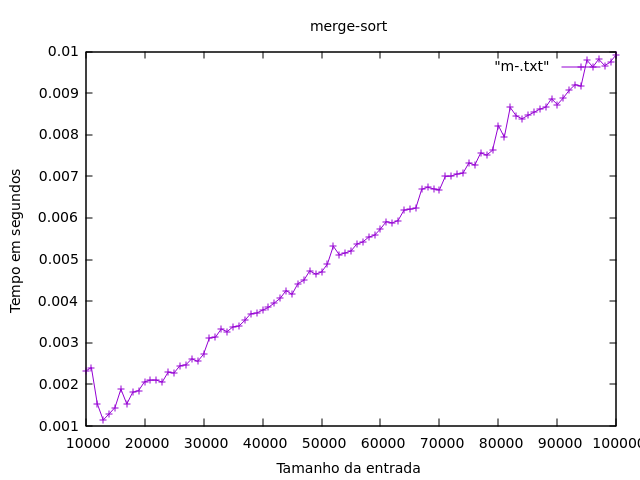
\includegraphics[width=1\linewidth]{Imagens/m-.png}
\end{figure}

\newpage

\section{Análise analítica do tempo de execução}

\subsection{Algoritmo}
\begin{figure}[h]
    \centering
    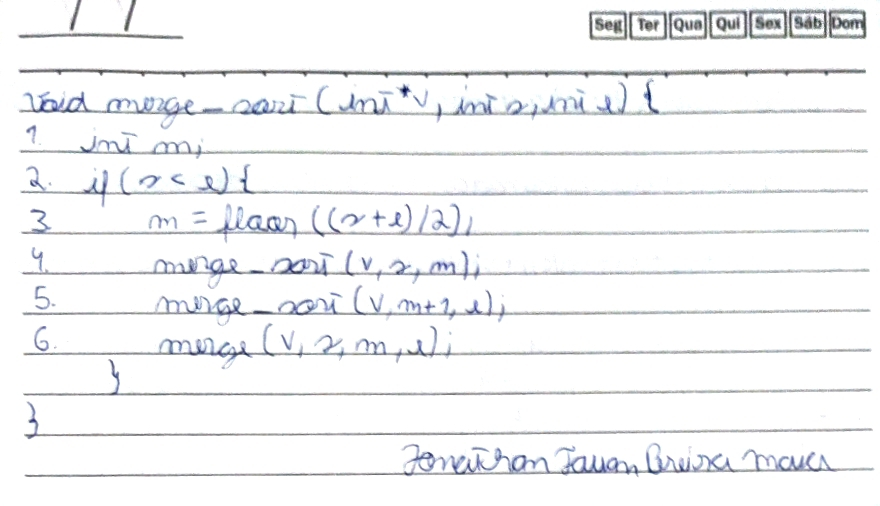
\includegraphics[width=0.76\linewidth]{Imagens/merge.jpg}
\end{figure}

\newpage
\subsubsection{Tempo esperado}
A análise analítica do tempo de execução do merge-sort permitiu perceber que em todos os casos o seu tempo de execução será sempre (n*log (n)).
\begin{figure}[h]
    \centering
    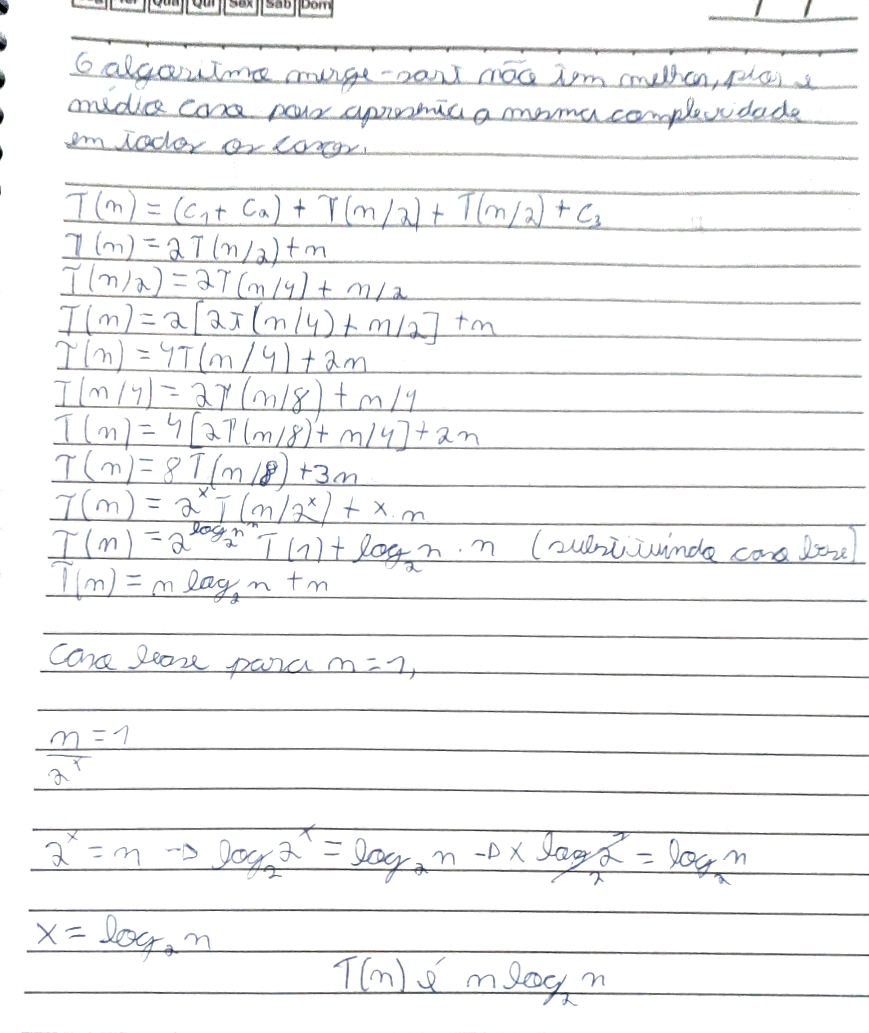
\includegraphics[width=0.76\linewidth]{Imagens/calculo-merge.jpg}
\end{figure}
	
	% Capitulo 4: Quarto capítulo (arquivo Includes/Capitulo4.tex)
	% Capítulo 4
\chapter{Quick Sort}
A função partition necessária para o funcionamento do quick-sort foi implementada pegando como pivô o último elemento da entrada para todos os casos.
\newpage
\section{Gráficos}
\subsection{Melhor caso}
O gráfico abaixo representa o tempo de execução do melhor caso do quick-sort em função do tamanho da entrada. Como entrada para gerar o gráfico, foram utilizados 91 vetores já ordenados, porém, com as posições do meio trocadas com a última posição para forçar o melhor caso. Pela análise do gráfico podemos notar que o algoritmo no melhor caso, desconsiderando a variação de tempo gerada por processos concorrentes no momento da execução do programa, pertence a O(n*log(n)).
\begin{figure}[h]
    \centering
    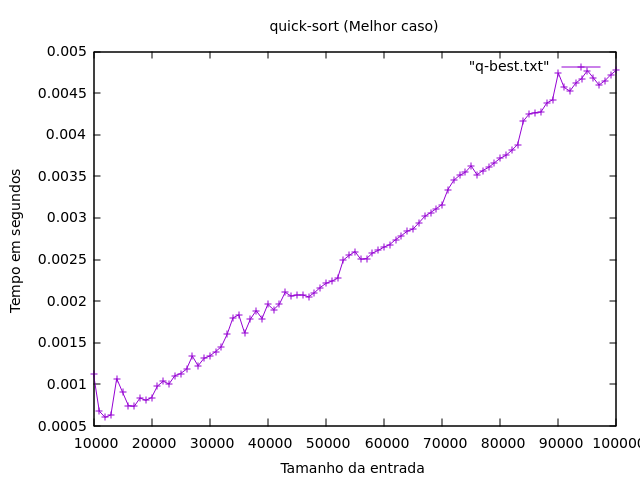
\includegraphics[width=1\linewidth]{Imagens/q-best.png}
\end{figure}

\newpage

\subsection{Pior caso}
O gráfico abaixo representa o tempo de execução do pior caso do quick-sort em função do tamanho da entrada. Como entrada para gerar o gráfico, foram utilizados 91 vetores já ordenados em ordem crescente. Pela análise do gráfico podemos notar que o algoritmo no pior caso, desconsiderando a variação de tempo gerada por processos concorrentes no momento da execução do programa, é quadrático. Tw(n) pertence a O(n²).
\begin{figure}[h]
    \centering
    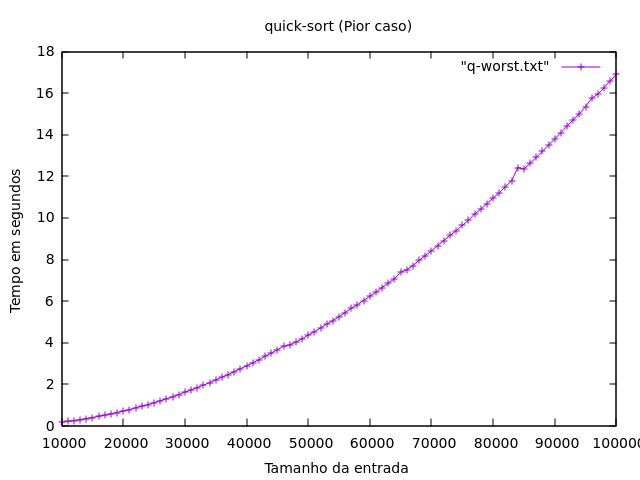
\includegraphics[width=1\linewidth]{Imagens/q-worst.png}
\end{figure}

\newpage

\subsection{Caso médio}
O gráfico abaixo representa o tempo de execução esperado do quick-sort em função do tamanho da entrada. Como entrada para gerar o gráfico, foram utilizados 91 vetores de tamanho n, preenchidos com números de 0 até n gerados aleatoriamente. Pela análise do gráfico podemos notar que o algoritmo no caso médio, desconsiderando a variação de tempo gerada por processos concorrentes no momento da execução do programa, pertence a O(n*log(n)).
\begin{figure}[h]
    \centering
    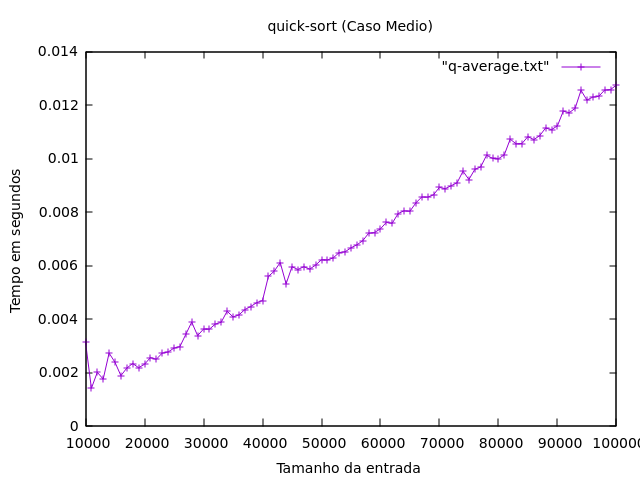
\includegraphics[width=1\linewidth]{Imagens/q-average.png}
\end{figure}

\newpage

\subsection{Comparação dos gráficos}
No gráfico abaixo podemos ver a comparação entre o caso médio, o melhor e o pior caso do algoritmo. É possível perceber que o tempo esperado e o melhor caso tem tempo muito inferior ao tempo do pior caso.
\begin{figure}[h]
    \centering
    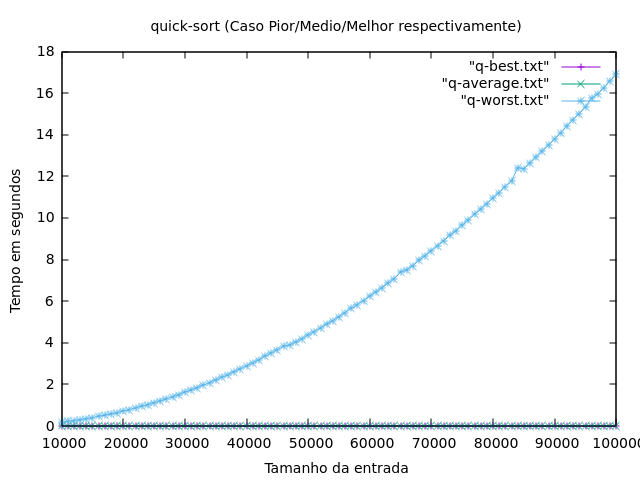
\includegraphics[width=1\linewidth]{Imagens/q-baw.png}
\end{figure}

\newpage

\section{Análise analítica do tempo de execução}
\subsection{Algoritmo}
\begin{figure}[h]
    \centering
    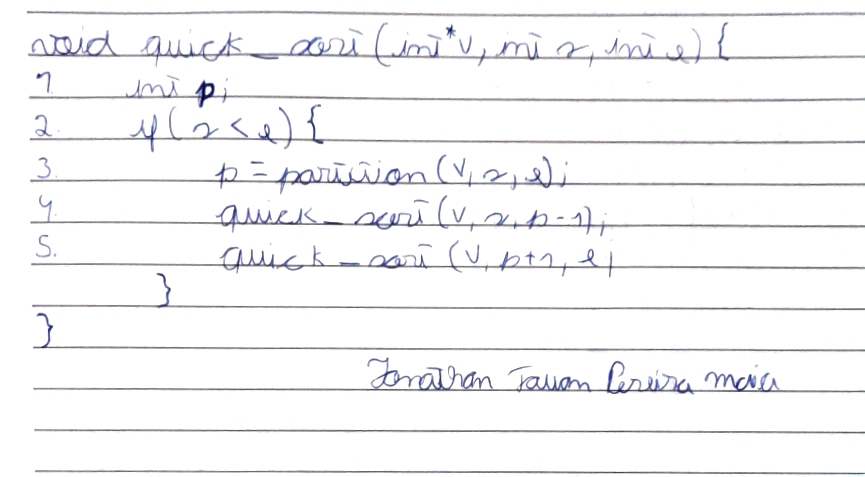
\includegraphics[width=0.76\linewidth]{Imagens/quick.jpg}
\end{figure}

\newpage

\subsubsection{Melhor caso}
A análise analítica do tempo de execução do quick-sort no seu melhor caso, que se dá quando o vetor já está ordenado, porém, com o elemento da posição do meio invertido com o último elemento do vetor, e temos como pivô a última posição, permitiu perceber que seu tempo de execução será (n*log (n)).
\begin{figure}[h]
    \centering
    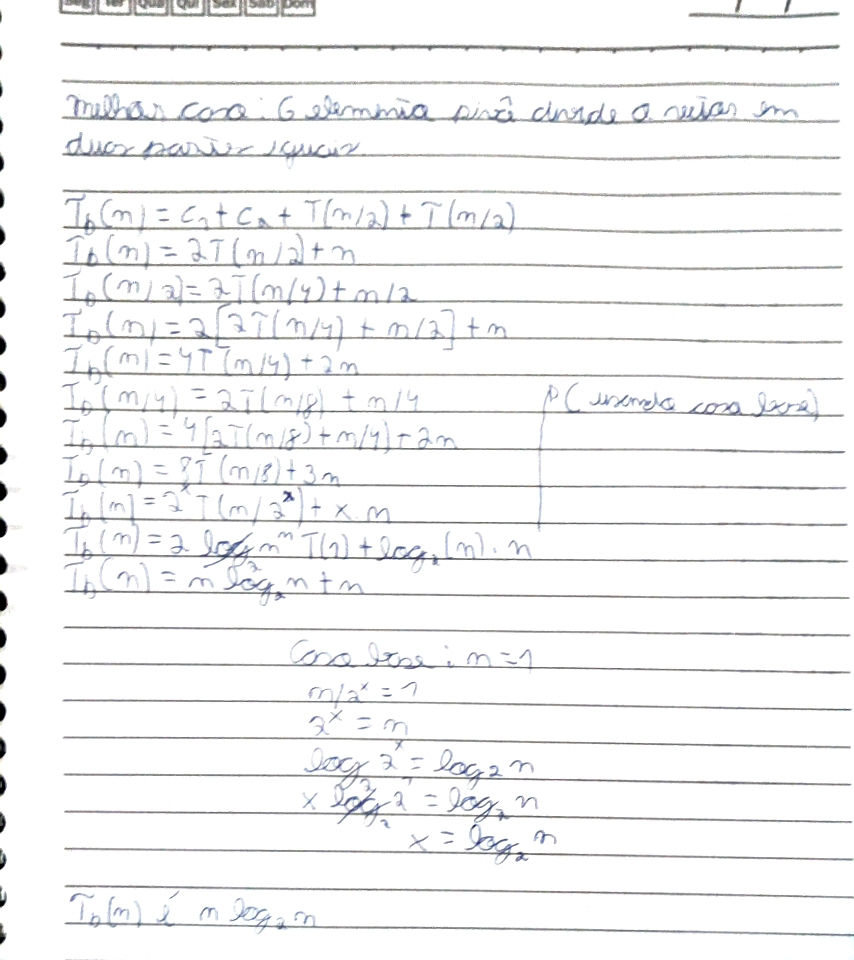
\includegraphics[width=0.76\linewidth]{Imagens/melhor-quick.jpg}
\end{figure}

\newpage

\subsubsection{Pior caso}
A análise analítica do tempo de execução do quick-sort no seu pior caso, que se dá quando o vetor já está ordenado, e pegamos o pivô também como o último elemento do vetor, permitiu perceber que seu tempo de execução será quadrático,  f(n) = an² +
bn + c.
\begin{figure}[h]
    \centering
    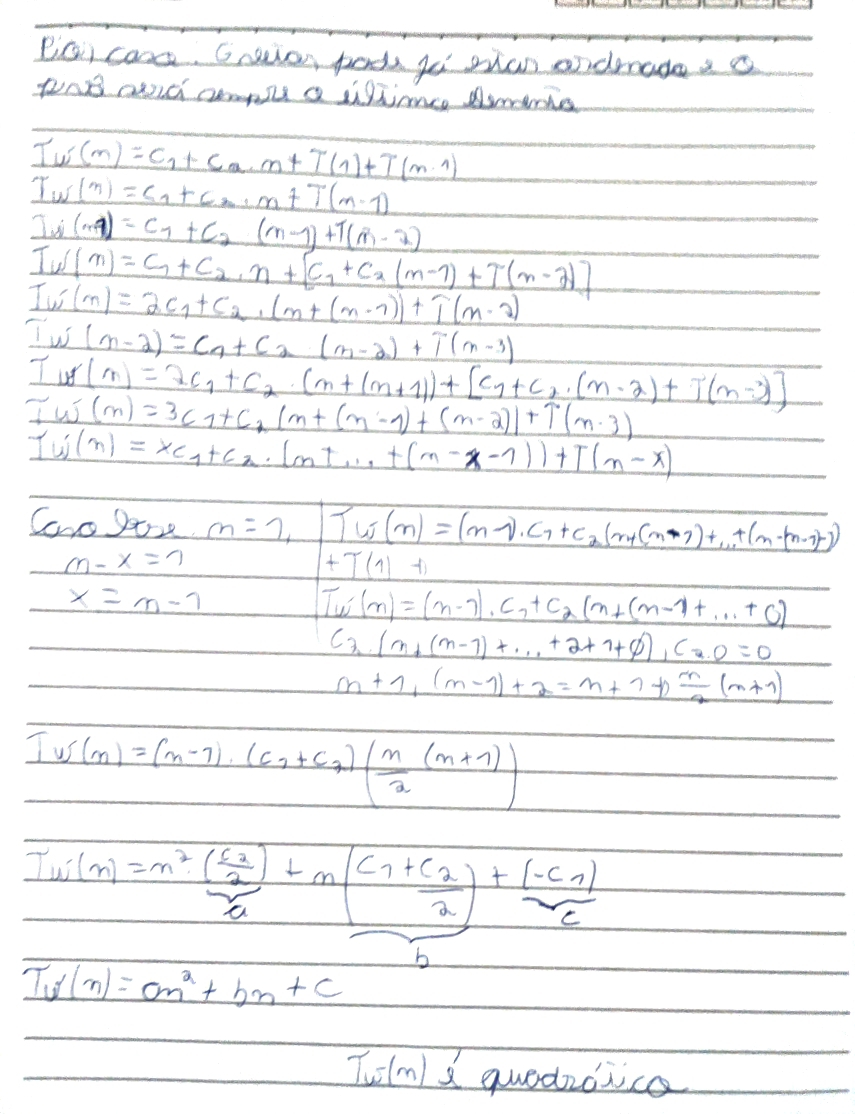
\includegraphics[width=0.76\linewidth]{Imagens/pior-quick.jpg}
\end{figure}
	
	% Capitulo 5: Quinto capítulo (arquivo Includes/Capitulo5.tex)
	% Capítulo 5
\chapter{Comparação de desempenho em relação ao custo de tempo e memória}
\subsection{Gráficos}
\subsubsection{Comparação do tempo esperado dos algoritmos}
O gráfico abaixo representa o tempo esperado dos três algortimos. É possível notar que o insertion-sort apresenta um tempo esperado muito maior do que os outros dois algoritmos.
\begin{figure}[h]
    \centering
    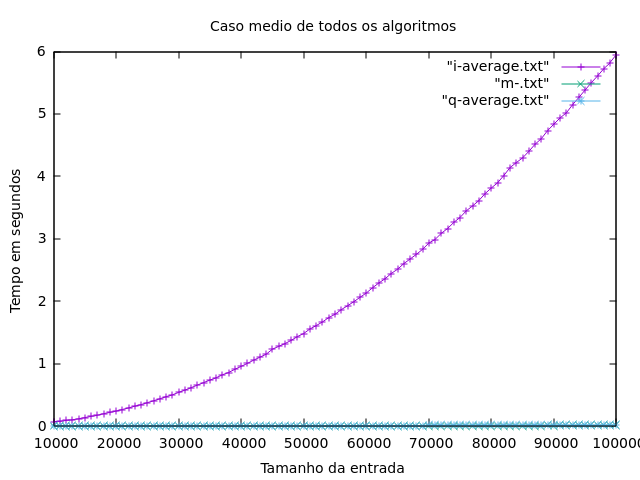
\includegraphics[width=1\linewidth]{Imagens/imq-average.png}
\end{figure}

\newpage
No gráfico abaixo excluímos o insertion-sort para podermos ver uma comparação melhor do tempo esperado do quick-sort com o tempo do merge-sort.
\begin{figure}[h]
    \centering
    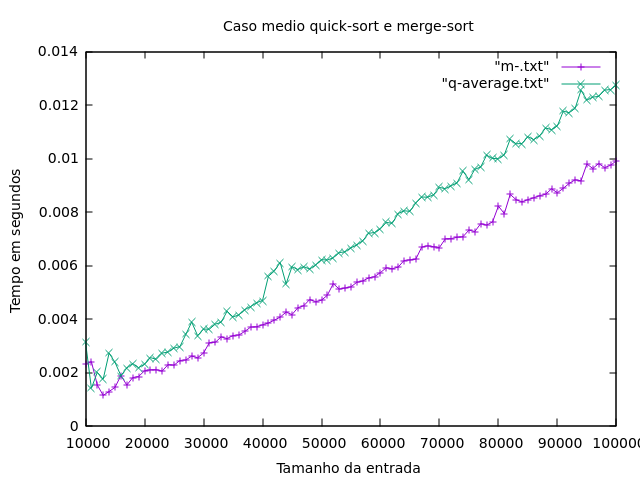
\includegraphics[width=1\linewidth]{Imagens/mq-average.png}
\end{figure}

\newpage
\subsubsection{Comparação do tempo do pior caso dos algoritmos}
Aqui abaixo temos a comparação do tempo do pior caso dos algoritmos quick-sort e insertion-sort com o o tempo do merge-sort.
\begin{figure}[h]
    \centering
    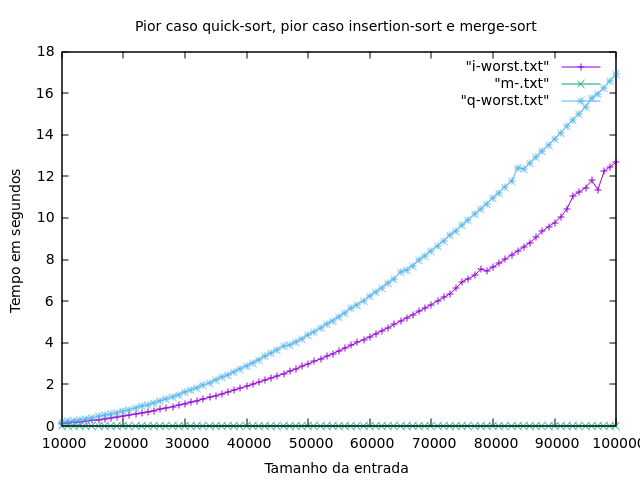
\includegraphics[width=1\linewidth]{Imagens/imq-worst.png}
\end{figure}

\newpage
\subsection{Conclusão}
Pela a análise dos gráficos de cada algoritmo levando em consideração seu melhor, pior e caso médio, foi possível observar que dentre os três, o algoritmo insertion-sort foi o que apresentou menor desempenho em relação ao tempo de execução esperado.

Porém, como não foi implementado de forma recursiva, o mesmo pode custar a menor quantidade de memória em comparação aos outros dois e seu pior caso ainda consegue ser melhor do que alguns casos específicos de pior caso do quick-sort.

Ainda analisando os algoritmos quick-sort e o merge-sort, podemos notar que, de acordo com o gráfico, o algoritmo quick-sort em seu melhor caso e seu caso médio, ainda é se apresentou rápido que o merge-sort.

Entretanto, o algoritmo merge-sort ainda se apresenta mais estável, pois, para todos os casos apresenta complexidade (n*log(n)), ao contrário do quick-sort que é volátil e mais instável, e apesar de ser mais rápido na maioria das vezes, no seu pior caso, pode chegar a complexidade de tempo O(n²), sendo bem inferior quando comparado ao tempo de execução do merge-sort.

Além disso, devemos considerar a implementação desses dois últimos de forma recursiva, que para grandes entradas podem apresentar uma sobrecarga na pilha de execução. Mas em relaçâo a memória, o quick-sort sai na frente pois o seu concorrente, o merge-sort, aloca um novo vetor a cada chamada recursiva da função merge, o que gera um gasto adicional e ainda mais notável em linguagens de mais alto nível.


\newpage
\subsubsection{Tabelas}

\centering
\caption{Melhor caso}
\begin{center}
\begin{tabular}{| l | r | r | r |}
\hline
& \multicolumn{3}{c|}{Tempo (s)}\\
\cline{2 - 4}
Tamanho da entrada & insertion-sort & merge-sort & quick-sort \\
\hline
10000 & 0.000043 & 0.002320 & 0.001124\\
20000 & 0.000057 & 0.002062 & 0.000842\\
30000 & 0.000084 & 0.002724 & 0.001341\\
40000 & 0.000126 & 0.003782 & 0.001962\\
50000 & 0.000193 & 0.004701 & 0.002213\\
\hline
\end{tabular}
\end{center}

\centering
\caption{Pior caso}
\begin{center}
\begin{tabular}{| l | r | r | r |}
\hline
& \multicolumn{3}{c|}{Tempo (s)}\\
\cline{2 - 4}
Tamanho da entrada & insertion-sort & merge-sort & quick-sort \\
\hline
10000 & 0.124559 & 0.002320 & 0.187187\\
20000 & 0.476691 & 0.002062 & 0.718812\\
30000 & 1.074601 & 0.002724 & 1.630973\\
40000 & 1.908465 & 0.003782 & 2.887971\\
50000 & 2.982496 & 0.004701 & 4.367089\\
\hline
\end{tabular}
\end{center}

\centering
\caption{Tempo esperado}
\begin{center}
\begin{tabular}{| l | r | r | r |}
\hline
& \multicolumn{3}{c|}{Tempo (s)}\\
\cline{2 - 4}
Tamanho da entrada & insertion-sort & merge-sort & quick-sort \\
\hline
10000 & 0.070669 & 0.002320 & 0.003140\\
20000 & 0.239225 & 0.002062 & 0.002307\\
30000 & 0.537542 & 0.002724 & 0.003623\\
40000 & 0.955588 & 0.003782 & 0.004691\\
50000 & 1.482152 & 0.004701 & 0.006215\\
\hline
\end{tabular}
\end{center}
	
	% Capitulo 6: Sexto capítulo (arquivo Includes/Capitulo6.tex)
	% Capítulo 6
\chapter{Diagrama de Casos de Uso}
\begin{figure}[h]
    \centering
    \includegraphics[width=1.0\linewidth]{Imagens/Sistema de empréstimos.pdf}
\end{figure}

\section{Descrição dos Atores}

\textbf{Usuário:} Este ator representa as pessoas físicas que mantém ou mantiveram contas na biblioteca, com direito a utilizar seus serviços como emprestimo de livros. Ele não acessa diretamente o sistema, mas se comunica com o funcionário para que esse realize as operações necessárias.\\\\

\textbf{Funcionário:} Este ator representa a pessoa física responsável pelo atendimento da biblioteca em determinado momento. Ele tem como função se relacionar com os usuários e lidar com a máquina que executa o sistema, realizando o resgistro de empréstimos e as demais possíveis operações com os materiais da biblioteca. Além disso, ele é encarregado  de manter todos os cadastros do sistema (funcionário, usuário, livro).
	
\section{Descrição dos Casos de Uso}

%Manter Usuário
\begin{longtable}{|l|}
\hline
\endfirsthead %% acaba o cabeçalho, ou primeira linha da coluna
\hline
\hline
\hline
\endhead
\hline \multicolumn{3}{r}{\emph{Continua na próxima página}}%%% isto aparecerá na quebra de página
\endfoot
\hline
\endlastfoot
Nome: Manter Usuário\\ \hline
Resumo: Caso de uso encarregado de adicionar, excluir, consultar e modificar os dados \\ de cada usuário. As informações necessárias para o cadastro são: Nome, CPF, RG,\\ telefone, endereço, data de nascimento e senha.\\ \hline
Pré-condição:  O usuário deve ter em mãos algum documento original com foto e CPF\\ para quaisquer operação no sistema (cadastro, exclusão, consulta, alteração e \\ empréstimos).\\ \hline
Pós-condição: Não se aplica.\\ \hline
Cenário principal:\\ \\ ADIÇÃO:\\        1. O funcionário solicita o documento e informações do usuário.\\        2. O usuário apresenta o documento e informa seus dados para o funcionário.\\        3. O funcionário insere no sistema as informações do usuário.\\         4. O funcionário conclui o cadastro salvando as informações.  \\ \\ CONSULTA:\\        1. O funcionário informa para o sistema o nome ou CPF do usuário.\\        2. O sistema exibe na tela todas as informações do usuário.\\ \\ EXCLUSÃO:\\        1. O funcionário consulta o cadastro do usuário (include consulta).\\        2. O funcionário clica na opção excluir cadastro.\\        3. O sistema exclui o usuário do cadastro de usuários.\\        4. O sistema exibe uma mensagem de sucesso.\\ \\ ALTERAÇÃO:\\        1. O funcionário solicita que o seu cadastro seja atualizado.\\        2. O funcionário solicita ao usuário o documento e as informações necessárias para \\atualização. \\        3. O funcionário localiza o cadastro do usuário no sistema (include consulta).\\        4. O funcionário altera as informações e salva no sistema.\\ \hline
Cenário alternativo:\\ \\ ADIÇÃO:\\ Documento do usuário é inválido.\\        \\ 3.1. Caso o documento do usuário seja inválido, ele será informado e deverá apresentar  \\ documentação válida.\\ \\Usuário é menor de idade.\\ \\3.1. Se o usuário for menor de idade não poderá ser cadastrado.\\ \\ CONSULTA:\\ Usuário não cadastrado.\\ \\ 2.1. Caso o usuário não esteja cadastrado o sistema será exibida a mensagem ¨Aluno\\ não encontrado¨.\\ \\ EXCLUSÃO:\\ Usuário com entrega de livro pendente.\\ \\ 3.1. Caso o usuário tenha algum empréstimo de livro ativo, não será possível realizar \\ a exclusão e uma mensagem será retornada ao funcionário. \\ \\ ALTERAÇÃO:\\ Documento do usuário é inválido.\\ \\ 3.1. Caso o documento do usuário seja inválido, ele será informado e deverá apresentar \\ documentação válida.\\ \hline
Requisitos não funcionais (restrições/validações):\\ \\         1. O CPF deverá ser composto por 11 dígitos.\\         2. O usuário deve ser maior de idade.\\ \hline
\end{longtable}

%Empréstimo ou Renovação
\begin{longtable}{|l|}
\hline
\endfirsthead %% acaba o cabeçalho, ou primeira linha da coluna
\hline
\hline
\hline
\endhead
\hline \multicolumn{3}{r}{\emph{Continua na próxima página}}%%% isto aparecerá na quebra de página
\endfoot
\hline
\endlastfoot
Nome: Empréstimo ou Renovação\\ \hline
Resumo: Caso de uso responsável por realizar ou renovar empréstimos de materiais  \\ solicitados pelo usuário. A movimentação será registrada no sistema junto com os dados \\ do usuário, identificação do material e data de devolução prevista.\\ \hline
Pré-condição: O usuário deve estar cadastrado no sistema. O usuário deve escolher um \\ livro que esteja disponível.\\ \hline
Pós-condição: Após o decorrer do período estipulado, o usuário deverá devolver ou \\ renovar o empréstimo do livro.\\ \hline
Cenário principal:\\ \\ EMPRÉSTIMO/RENOVAÇÃO:\\        1. O usuário deve escolher um livro para empréstimo.\\        2. O usuário deve ser atendido pelo funcionário para realizar o empréstimo.\\        3. O usuário deve apresentar documento com foto e seus dados para ser localizado\\ no sistema. \\         4. O funcionário registra a movimentação no sistema e informa a data de devolução \\ para o usuário. \\         5. O usuário digita a senha. \\         6. O usuário retira o livro e o atendimento é encerrado. \\ \hline
Cenário alternativo:\\ \\ EMPRÉSTIMO/RENOVAÇÃO:\\ Usuário com cadastro inválido.\\        \\ 3.1. O usuário que não possui cadastro ou cadastro inválido é convidado a fazer ou  \\ atualizar o cadastro (extends manter usuário -> adição ou alteração ).\\ \\Usuário com pendências.\\ \\4.1. O usuário já tem o máximo de livros emprestados nesse momento (3) ou o usuário já\\ possui o mesmo livro emprestado atualmente ou o usuário possui livros com empréstimos\\ vencidos. O usuário é avisado ou penalizado e o caso de uso é encerrado.\\  \\Usuário informa senha errada.\\ \\6.1. É solicitado a senha novamente ao usuário por 3 vezes no máximo.\\ 6.2. Caso o usuário não saiba a senha, o funcionário ajuda-o a recupera-lá. O usuário\\ deve informar seus dados e apresentar documento válido.\\ \hline
Requisitos não funcionais (restrições/validações):\\ \\         1. O usuário deve estar cadastrado no sistema.\\         2. O usuário não poderá ter mais de 3 livros emprestados simultaneamente.\\         3. O usuário deverá informar senha válida. \hline
\end{longtable}

% Manter Livro
\begin{longtable}{|l|}
\hline
\endfirsthead %% acaba o cabeçalho, ou primeira linha da coluna
\hline
\hline
\hline
\endhead
\hline \multicolumn{3}{r}{\emph{Continua na próxima página}}%%% isto aparecerá na quebra de página
\endfoot
\hline
\endlastfoot
Nome: Manter Livro\\ \hline
Resumo: Caso de uso encarregado de adicionar, excluir, consultar e modificar os dados \\ de cada livro. As informações necessárias para o cadastro são: Nome, autor e editora.\\ \hline
Pré-condição: O funcionário deve ter em mãos alguma informação sobre o livro para\\ quaisquer operação no sistema (cadastro, exclusão, consulta, alteração e empréstimos).\\ \hline
Pós-condição: Não se aplica.\\ \hline
Cenário principal:\\ \\ ADIÇÃO:\\        1. O funcionário verifica informações do livro.\\        2. O funcionário insere no sistema as informações do livro.\\        3. O funcionário conclui o cadastro salvando as informações.\\ \\ CONSULTA:\\        1. O funcionário informa para o sistema o nome do livro.\\        2. O sistema exibe na tela todas as informações do livro.\\ \\ EXCLUSÃO:\\        1. O funcionário consulta o cadastro do livro (include consulta).\\        2. O funcionário clica na opção excluir cadastro.\\        3. O sistema exclui o livro do cadastro de livros.\\        4. O sistema exibe uma mensagem de sucesso.\\ \\ ALTERAÇÃO:\\        1. O funcionário solicita que o seu cadastro seja atualizado.\\        2. O funcionário insere as informações necessárias sobre o livro para atualização.\\        3. O funcionário localiza o cadastro do livro no sistema (include consulta).\\        4. O funcionário altera as informações e salva no sistema.\\ \hline
Cenário alternativo:\\ \\ ADIÇÃO:\\ Informações do livro são inválidas.\\        \\ 2.1. Caso as informações do livro sejam inválidas, o funcionário será informado e deverá \\ apresentar informações válidas.\\ \\ CONSULTA:\\ Livro não cadastrado.\\ \\ 2.1. Caso o livro não esteja cadastrado o sistema será exibida a mensagem "Livro não\\ encontrado".\\ \\ EXCLUSÃO:\\ Usuário com entrega de livro pendente.\\ \\ 3.1. Caso o livro tenha algum empréstimo ativo, não será possível realizar a exclusão.\\ \\ ALTERAÇÃO:\\ Informações do livro são inválidas.\\ \\ 3.1. Caso as informações do livro sejam inválidas, o funcionário será informado e deverá\\ apresentar informações válidas.\\ \hline
Requisitos não funcionais (restrições/validações):\\ \\ Não se aplica.\\ \hline
\end{longtable}

%Manter Funcionário
\begin{longtable}{|l|}
\hline
\endfirsthead %% acaba o cabeçalho, ou primeira linha da coluna
\hline
\hline
\hline
\endhead
\hline \multicolumn{3}{r}{\emph{Continua na próxima página}}%%% isto aparecerá na quebra de página
\endfoot
\hline
\endlastfoot
Nome: Manter Funcionário\\ \hline
Resumo: Caso de uso encarregado de adicionar, excluir, consultar e modificar os dados \\ de cada funcionário. As informações necessárias para cadastro são: nome, CPF, RG, \\ telefone, endereço, data de nascimento, salário, função.\\ \hline
Pré-condição:  O funcionário deve ter em mãos algum documento original com foto e CPF\\ para quaisquer operação no sistema (cadastro, exclusão, consulta, alteração e \\ empréstimos).\\ \hline
Pós-condição: Não se aplica.\\ \hline
Cenário principal:\\ \\ ADIÇÃO:\\        1. O funcionário solicita o documento e informações do funcionário.\\        2. O funcionário apresenta o documento e informa seus dados para o funcionário.\\        3. O funcionário insere no sistema as informações do funcionário.\\         4. O funcionário conclui o cadastro salvando as informações.  \\ \\ CONSULTA:\\        1. O funcionário informa para o sistema o nome ou CPF do funcionário.\\        2. O sistema exibe na tela todas as informações do funcionário.\\ \\ EXCLUSÃO:\\        1. O funcionário consulta o cadastro do funcionário (include consulta).\\        2. O funcionário clica na opção excluir cadastro.\\        3. O sistema exclui o funcionário do cadastro de funcionários.\\        4. O sistema exibe uma mensagem de sucesso.\\ \\ ALTERAÇÃO:\\        1. O funcionário solicita que o seu cadastro seja atualizado.\\        2. O funcionário solicita ao funcionário o documento e as informações necessárias para \\atualização. \\        3. O funcionário localiza o cadastro do funcionário no sistema (include consulta).\\        4. O funcionário altera as informações e salva no sistema.\\ \hline
Cenário alternativo:\\ \\ ADIÇÃO:\\ Documento do funcionário é inválido.\\        \\ 3.1. Caso o documento do funcionário seja inválido, ele será informado e deverá apresentar  \\ documentação válida.\\ \\funcionário é menor de idade.\\ \\3.1. Se o funcionário for menor de idade não poderá ser cadastrado.\\ \\ CONSULTA:\\ funcionário não cadastrado.\\ \\ 2.1. Caso o funcionário não esteja cadastrado o sistema será exibida a mensagem ¨funcionário\\ não encontrado¨.\\ \\ ALTERAÇÃO:\\ Documento do funcionário é inválido.\\ \\ 3.1. Caso o documento do funcionário seja inválido, ele será informado e deverá apresentar \\ documentação válida.\\ \hline
Requisitos não funcionais (restrições/validações):\\ \\         1. O CPF deverá ser composto por 11 dígitos.\\         2. O funcionário deve ser maior de idade.\\ \hline
\end{longtable}
	
	% Capitulo 7: Sétimo capítulo (arquivo Includes/Capitulo7.tex)
	% Capítulo 7
\chapter{Diagrama de Classes}
\begin{figure}[h]
    \centering
    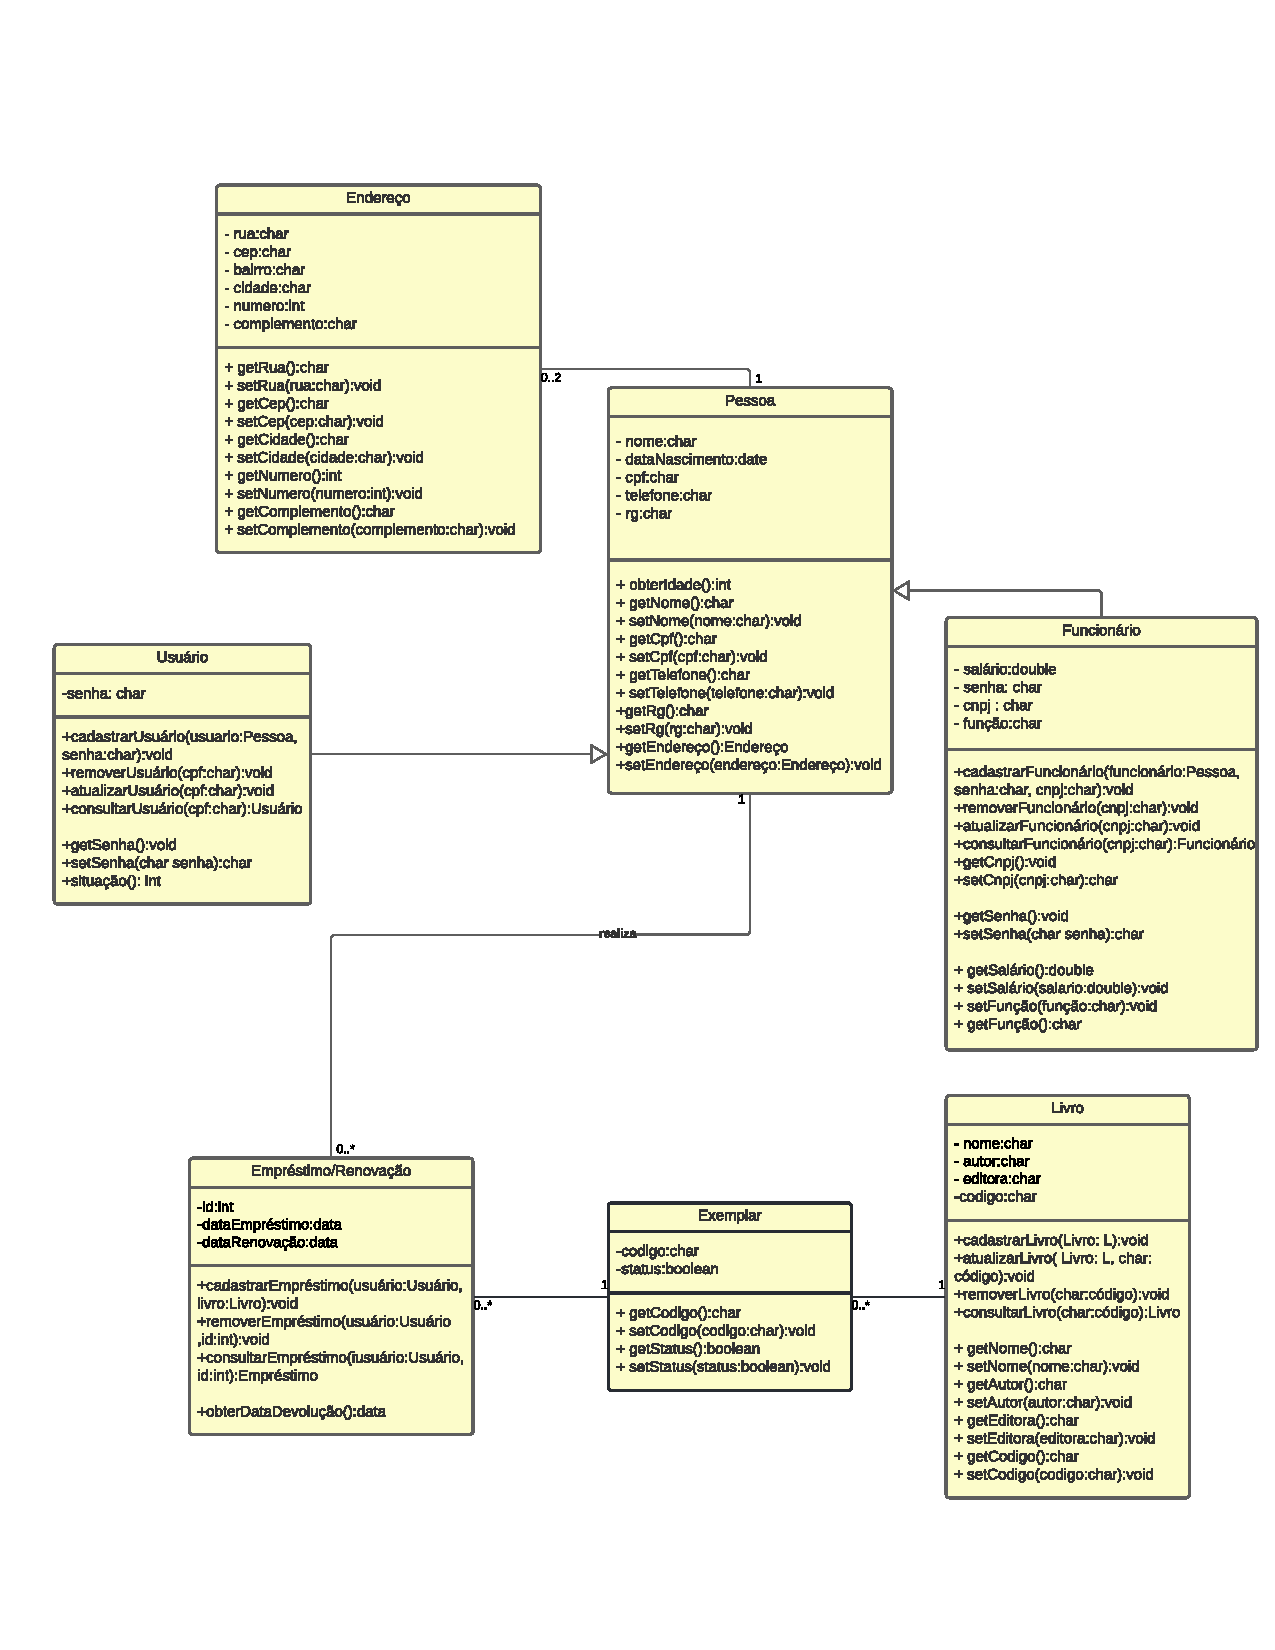
\includegraphics[width=0.8\linewidth]{Imagens/diagramadeclasses.pdf}
\end{figure}
	
	% Capitulo 8: Oitavo capítulo (arquivo Includes/Capitulo8.tex)
	% Capítulo 8
\chapter{Diagramas de Sequência}

\section{Manter Usuário} 

\subsection{Cadastro}

\begin{figure}[h]
    \centering
    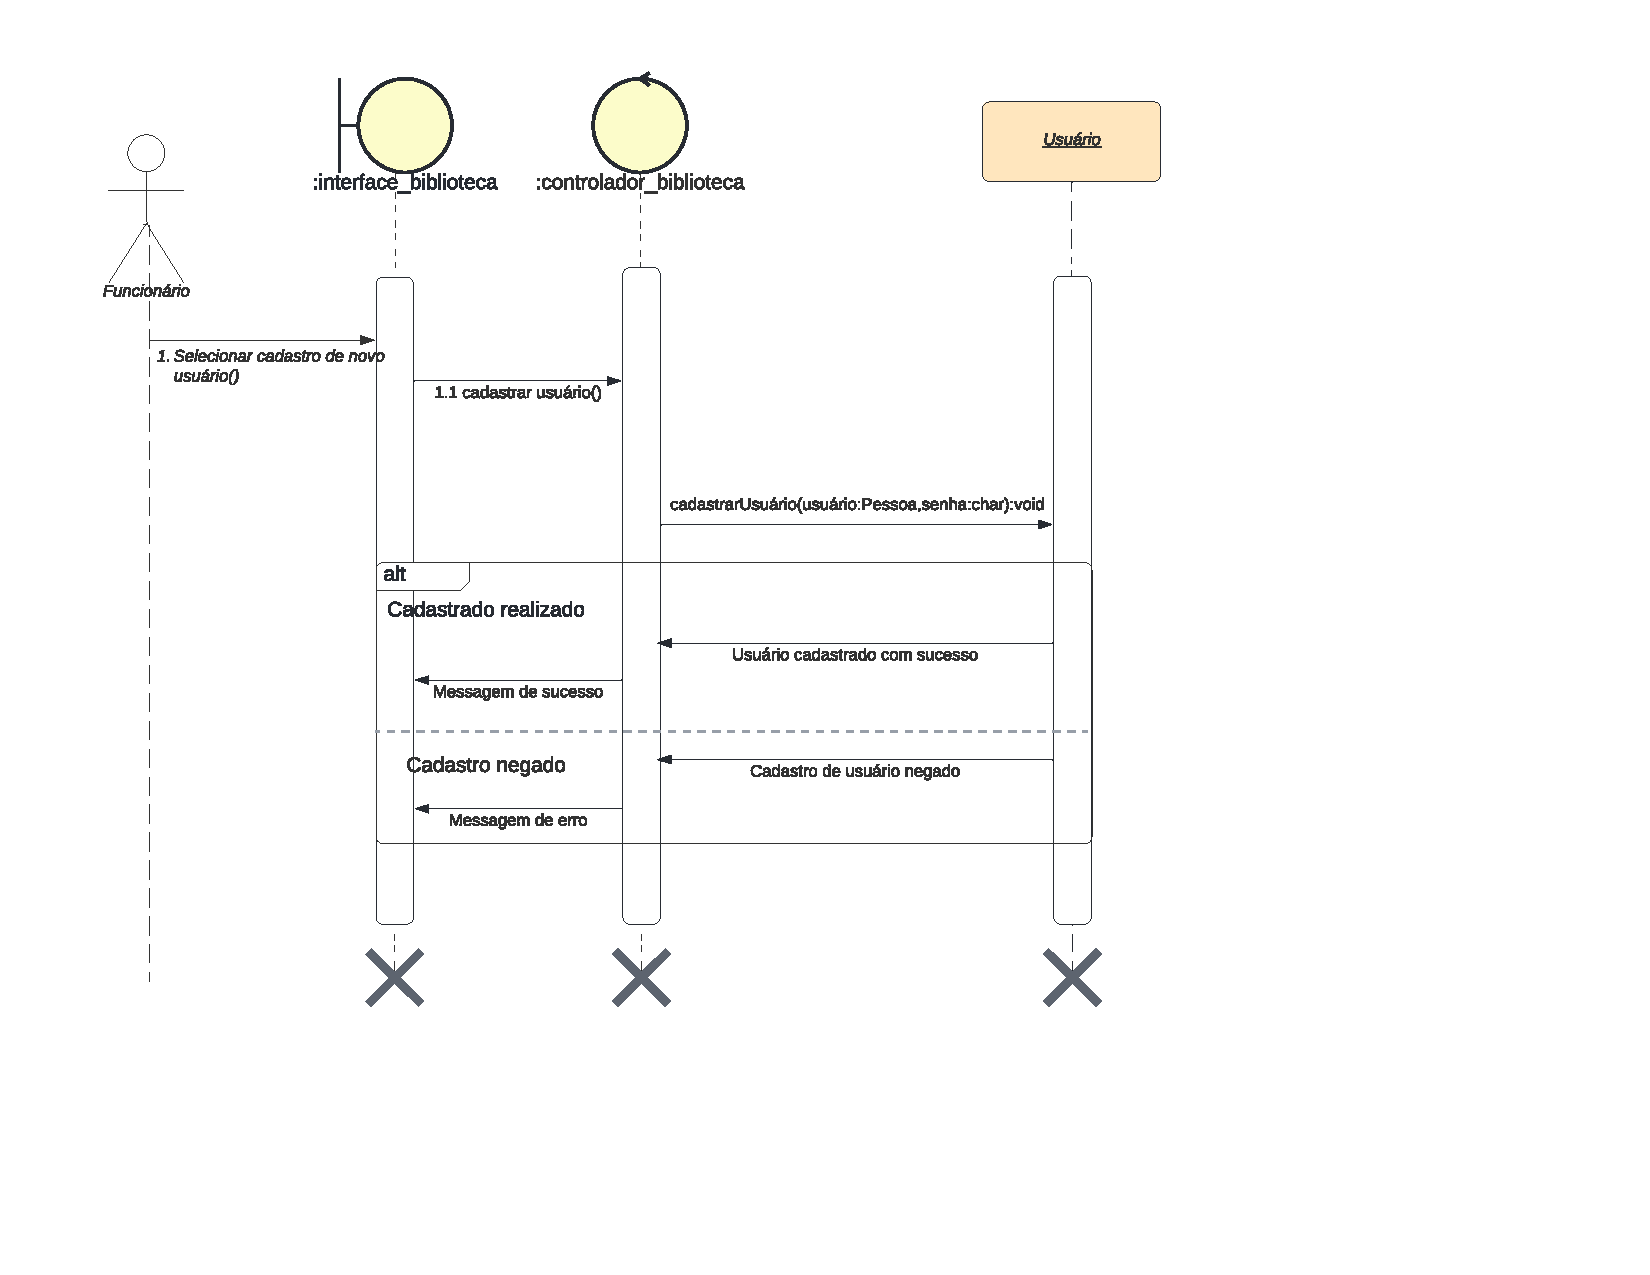
\includegraphics[width=1.0\linewidth]{Imagens/CadastrarUsuario-sequencia.pdf}
\end{figure}

\newpage

\subsection{Consulta}

\begin{figure}[h]
    \centering
    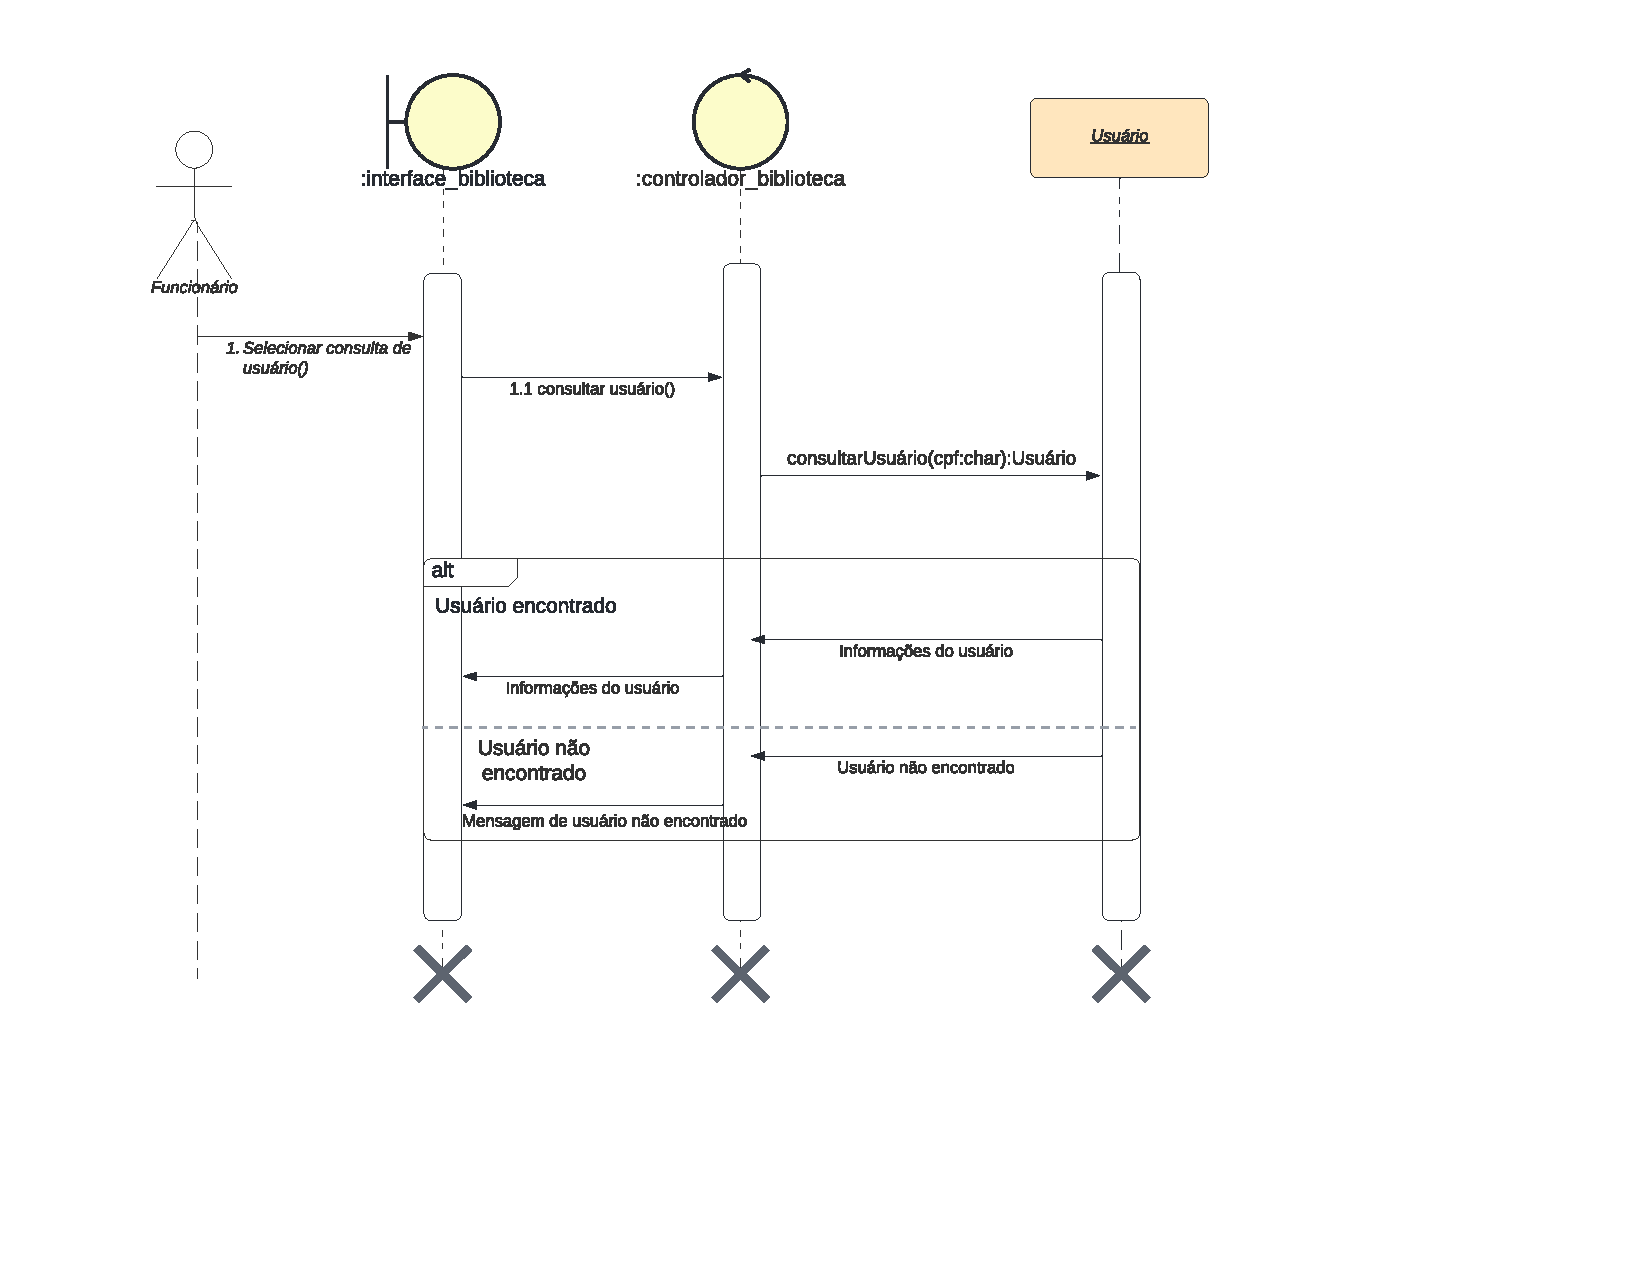
\includegraphics[width=1.0\linewidth]{Imagens/ConsultarUsuario-sequencia.pdf}
\end{figure}

\newpage

\subsection{Exclusão}

\begin{figure}[h]
    \centering
    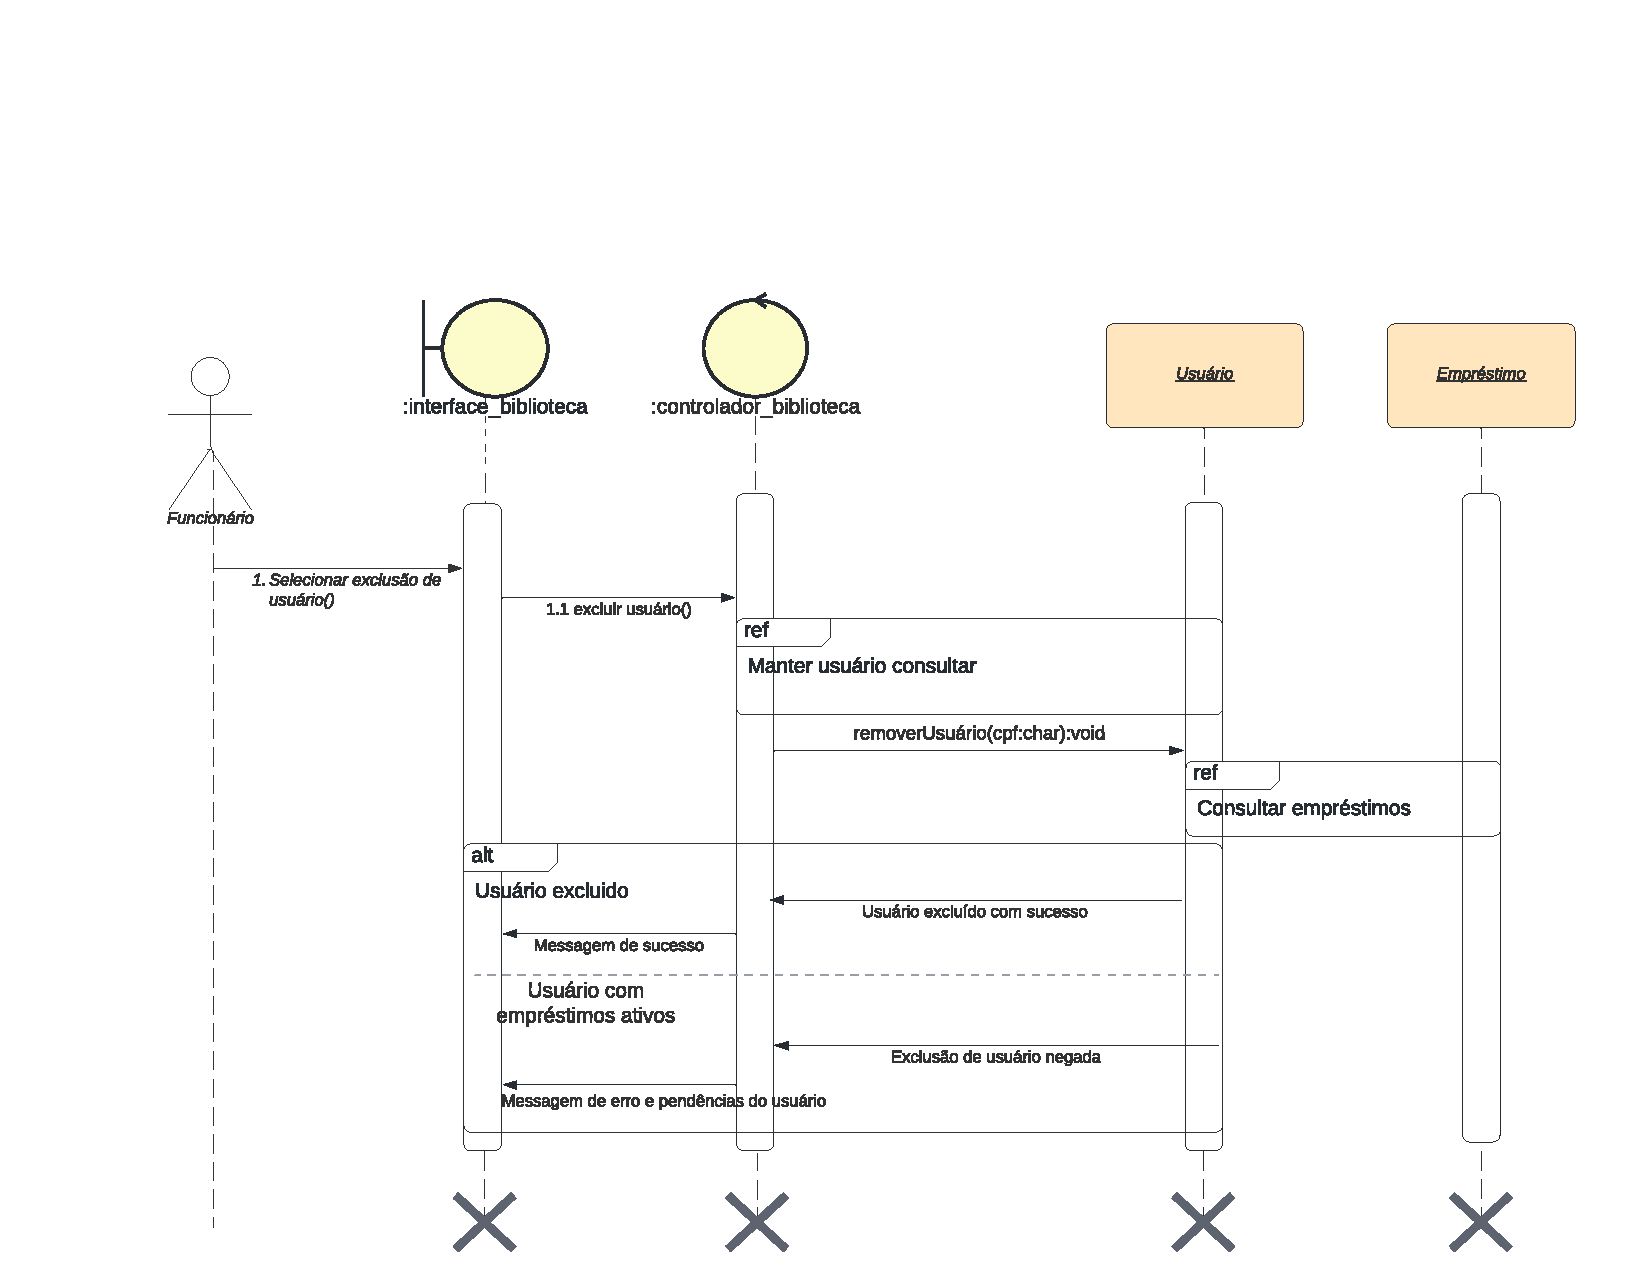
\includegraphics[width=1.0\linewidth]{Imagens/ExcluirUsuario-sequencia.pdf}
\end{figure}

\newpage

\subsection{Alteração}

\begin{figure}[h]
    \centering
    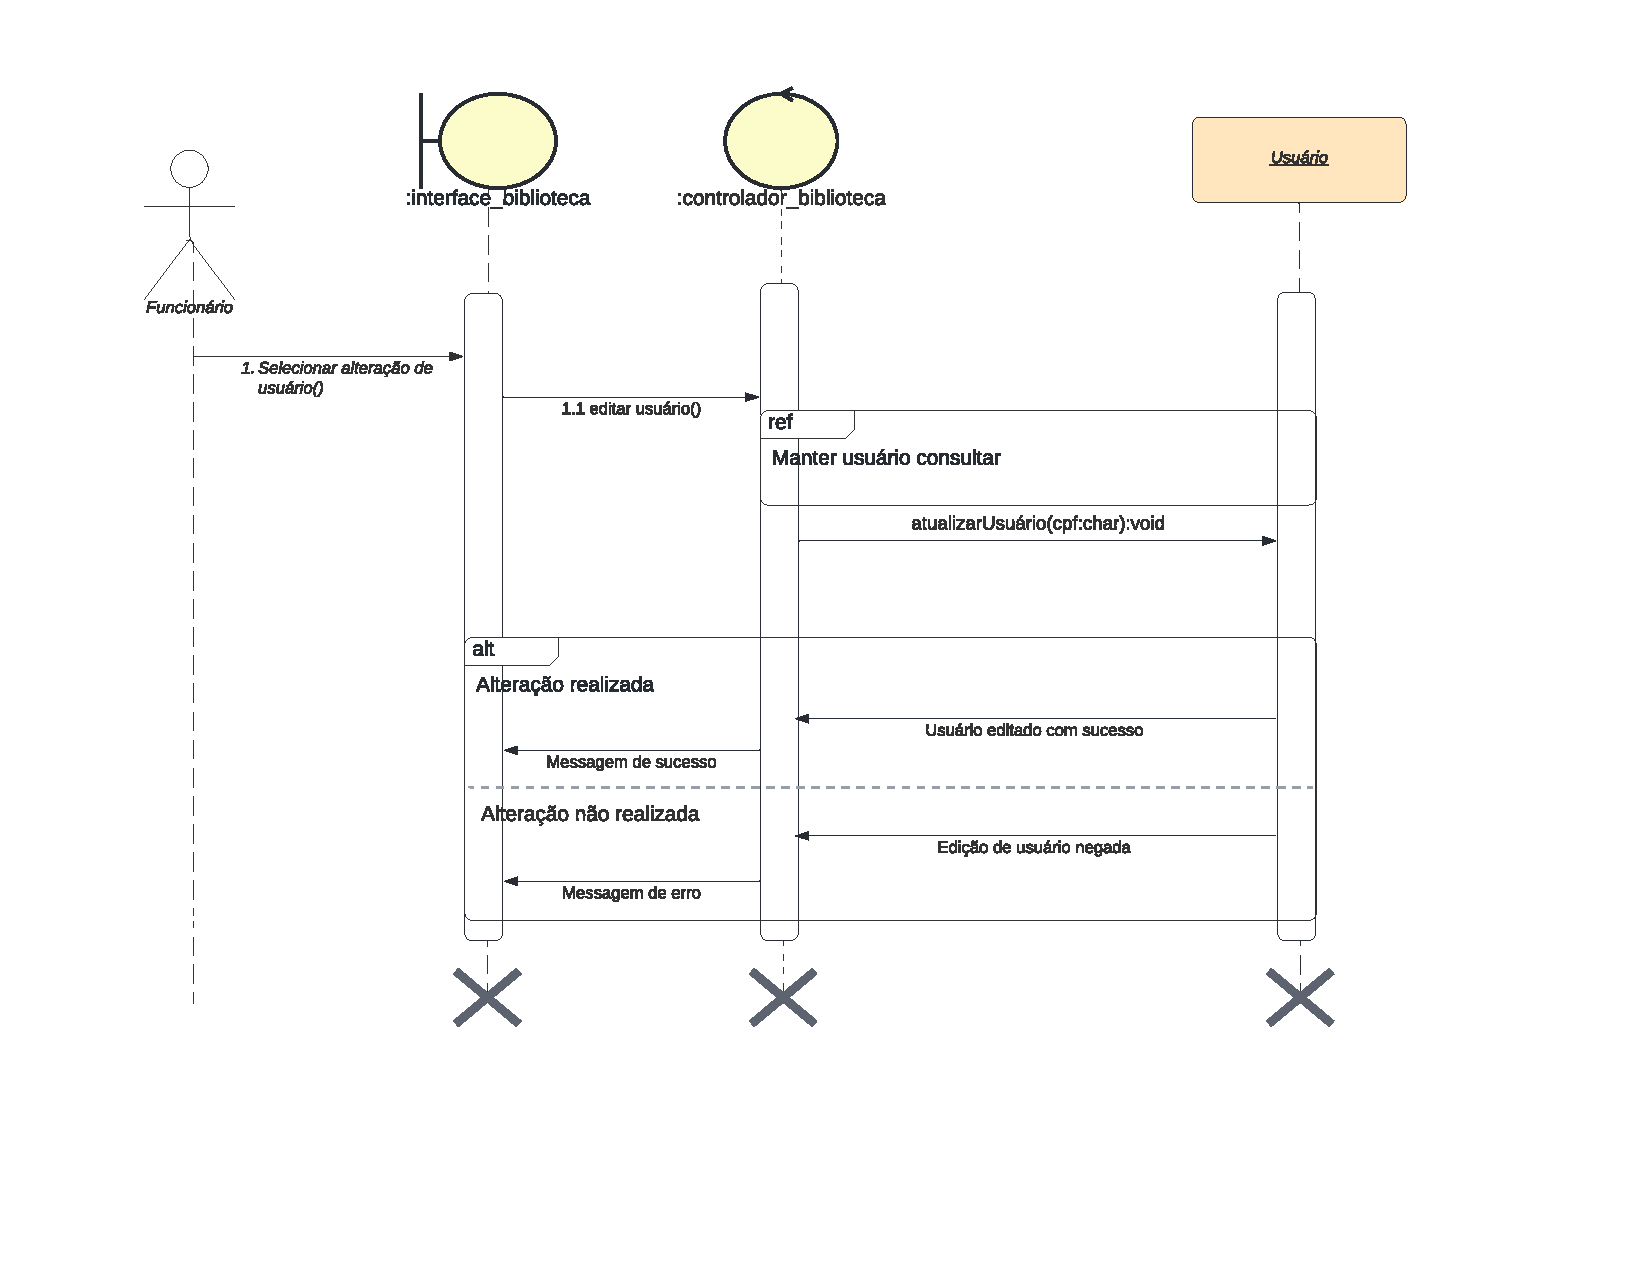
\includegraphics[width=1.0\linewidth]{Imagens/AlterarUsuario-sequencia.pdf}
\end{figure}

\newpage

%%%%%%%%%%%%%%%%%%%%%%%%%%%%%%%%%%%%%%%%%%%%%%%%%%%%%%%%%%%%%%%%%%%%%%%%%%%%%%%%%%%%%%%%%%%%%%%%%%%%%

\section{Empréstimo} 

\begin{figure}[h]
    \centering
    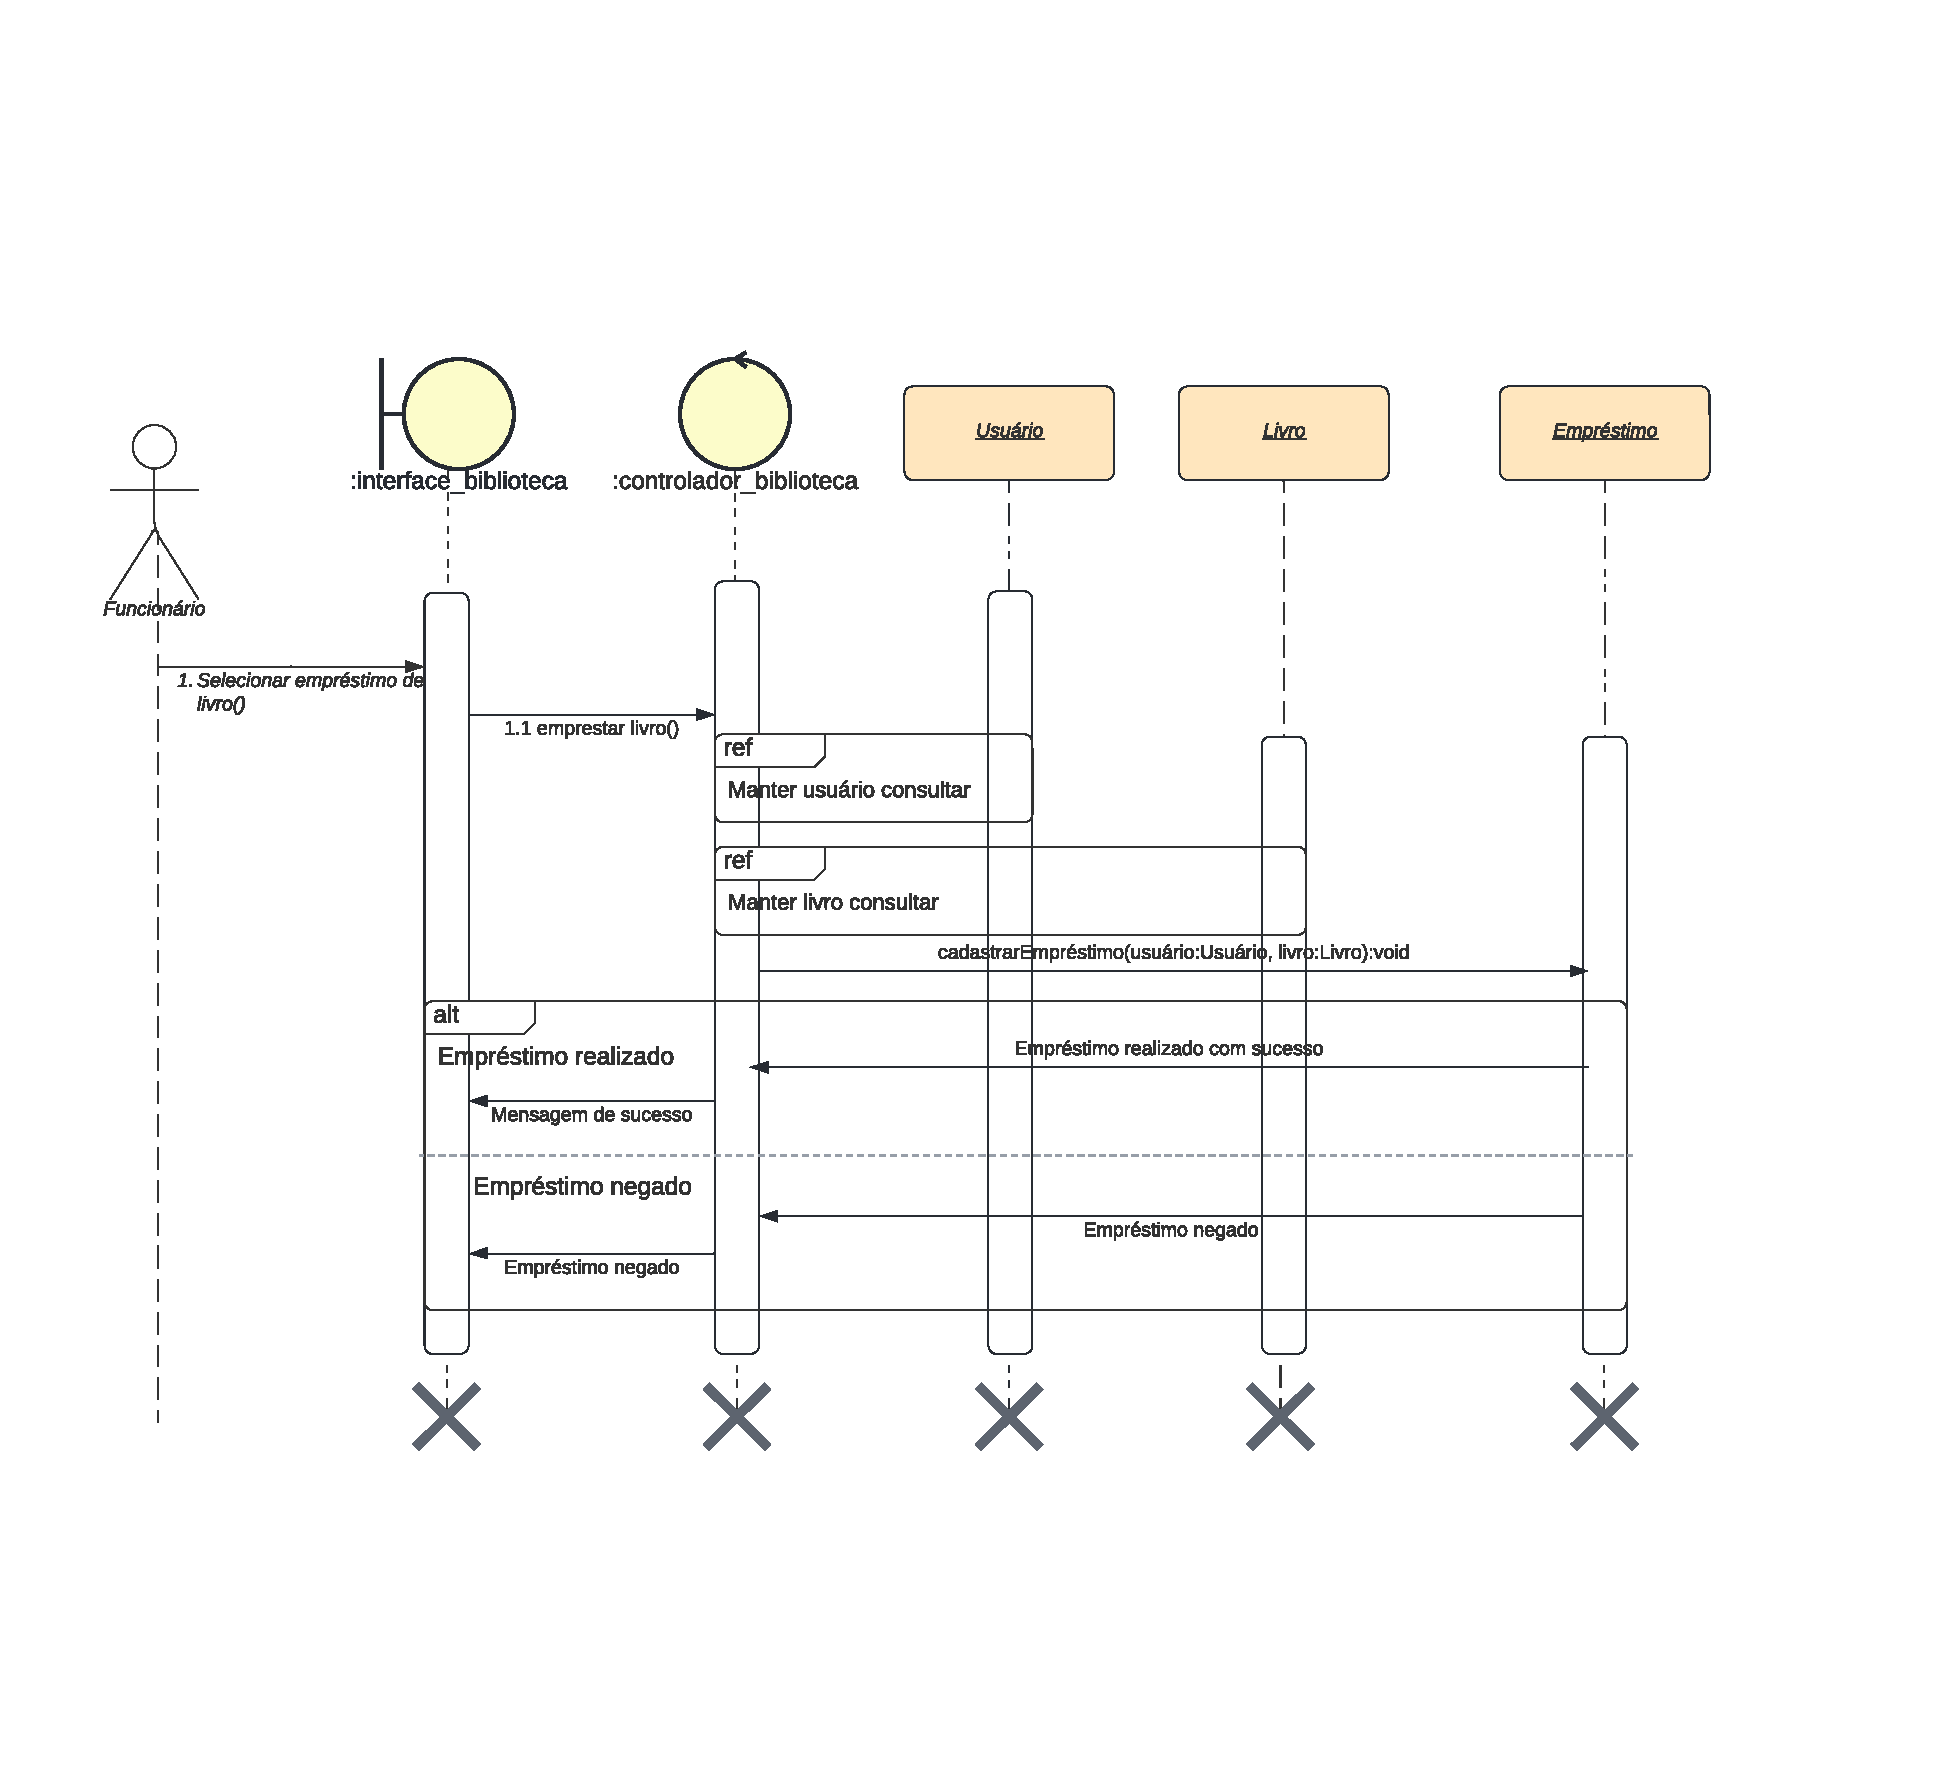
\includegraphics[width=1.0\linewidth]{Imagens/Emprestimo-sequencia.pdf}
\end{figure}

\newpage

%%%%%%%%%%%%%%%%%%%%%%%%%%%%%%%%%%%%%%%%%%%%%%%%%%%%%%%%%%%%%%%%%%%%%%%%%%%%%%%%%%%%%%%%%%%%%%%%%%%%%

\section{Manter Livro} 

\subsection{Cadastro}

\begin{figure}[h]
    \centering
    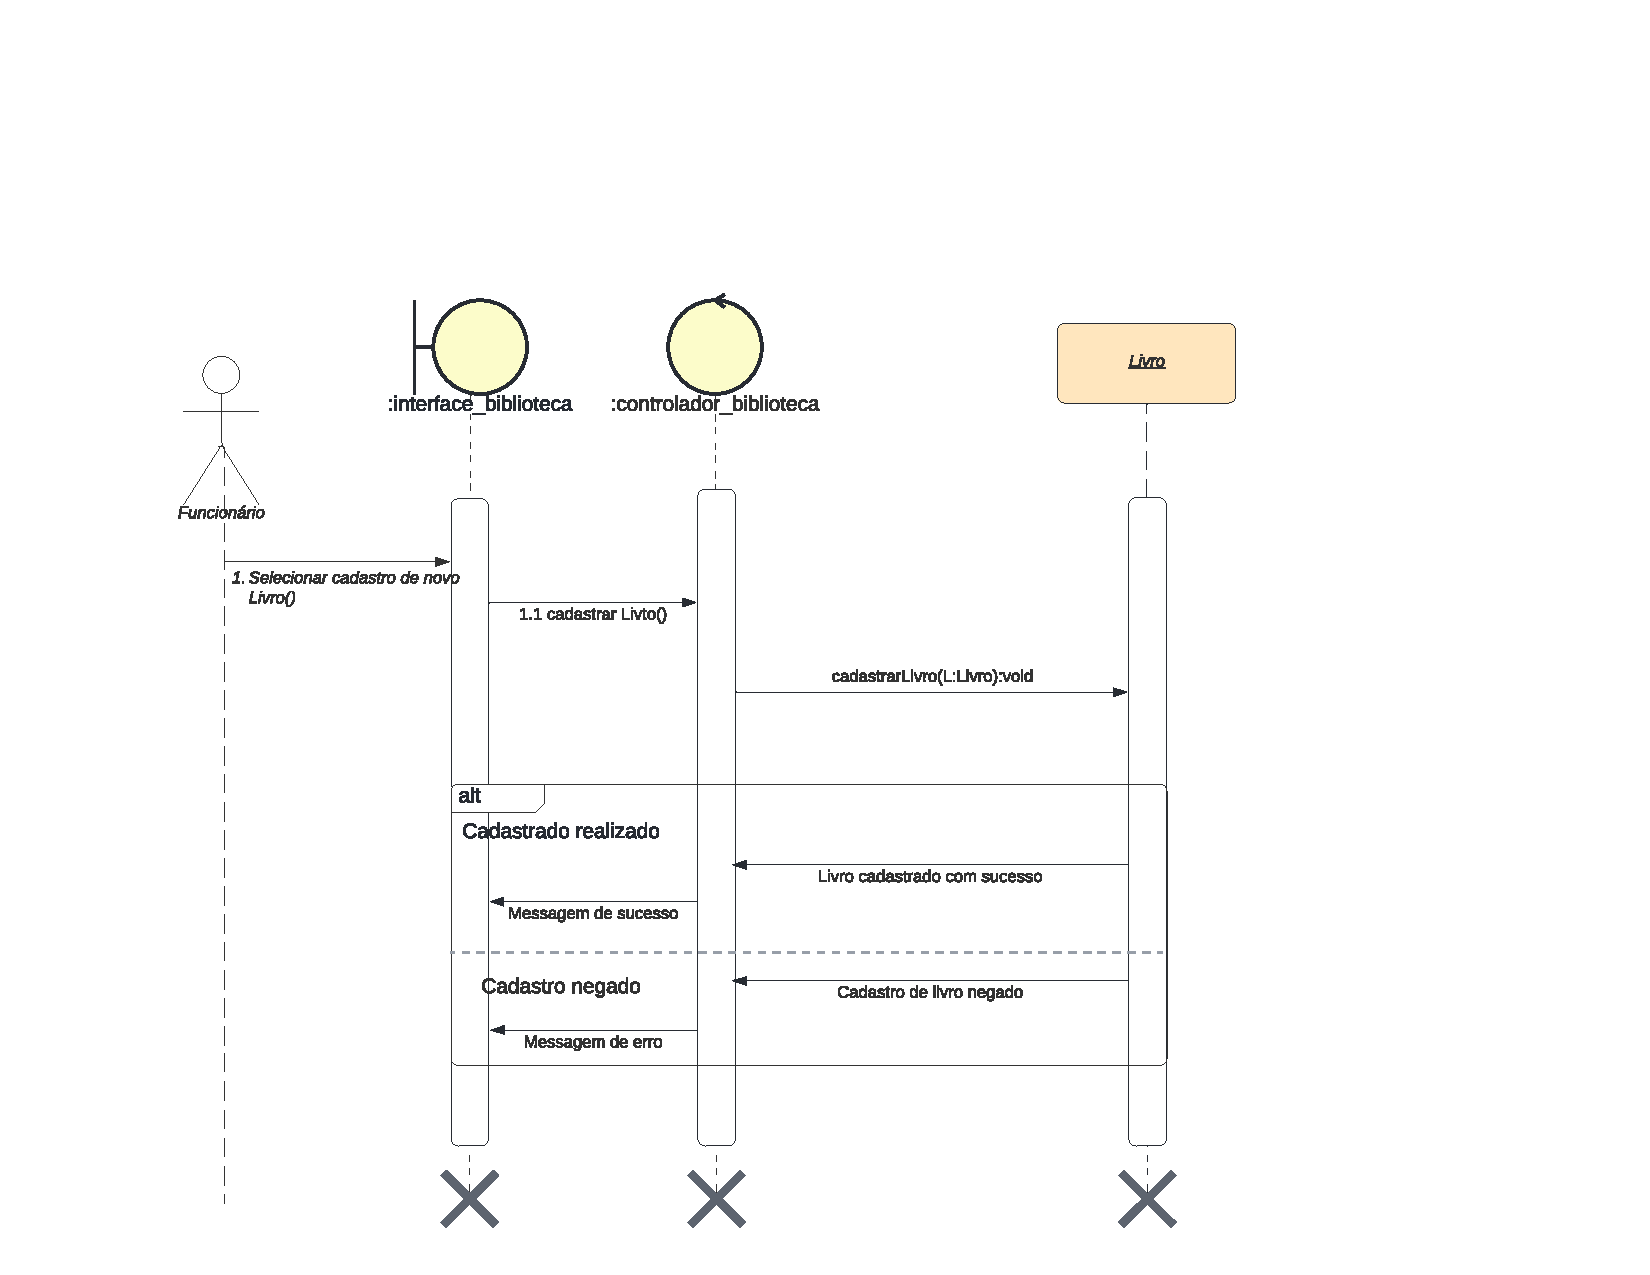
\includegraphics[width=1.0\linewidth]{Imagens/CadastrarLivro-sequencia.pdf}
\end{figure}

\newpage

\subsection{Consulta}

\begin{figure}[h]
    \centering
    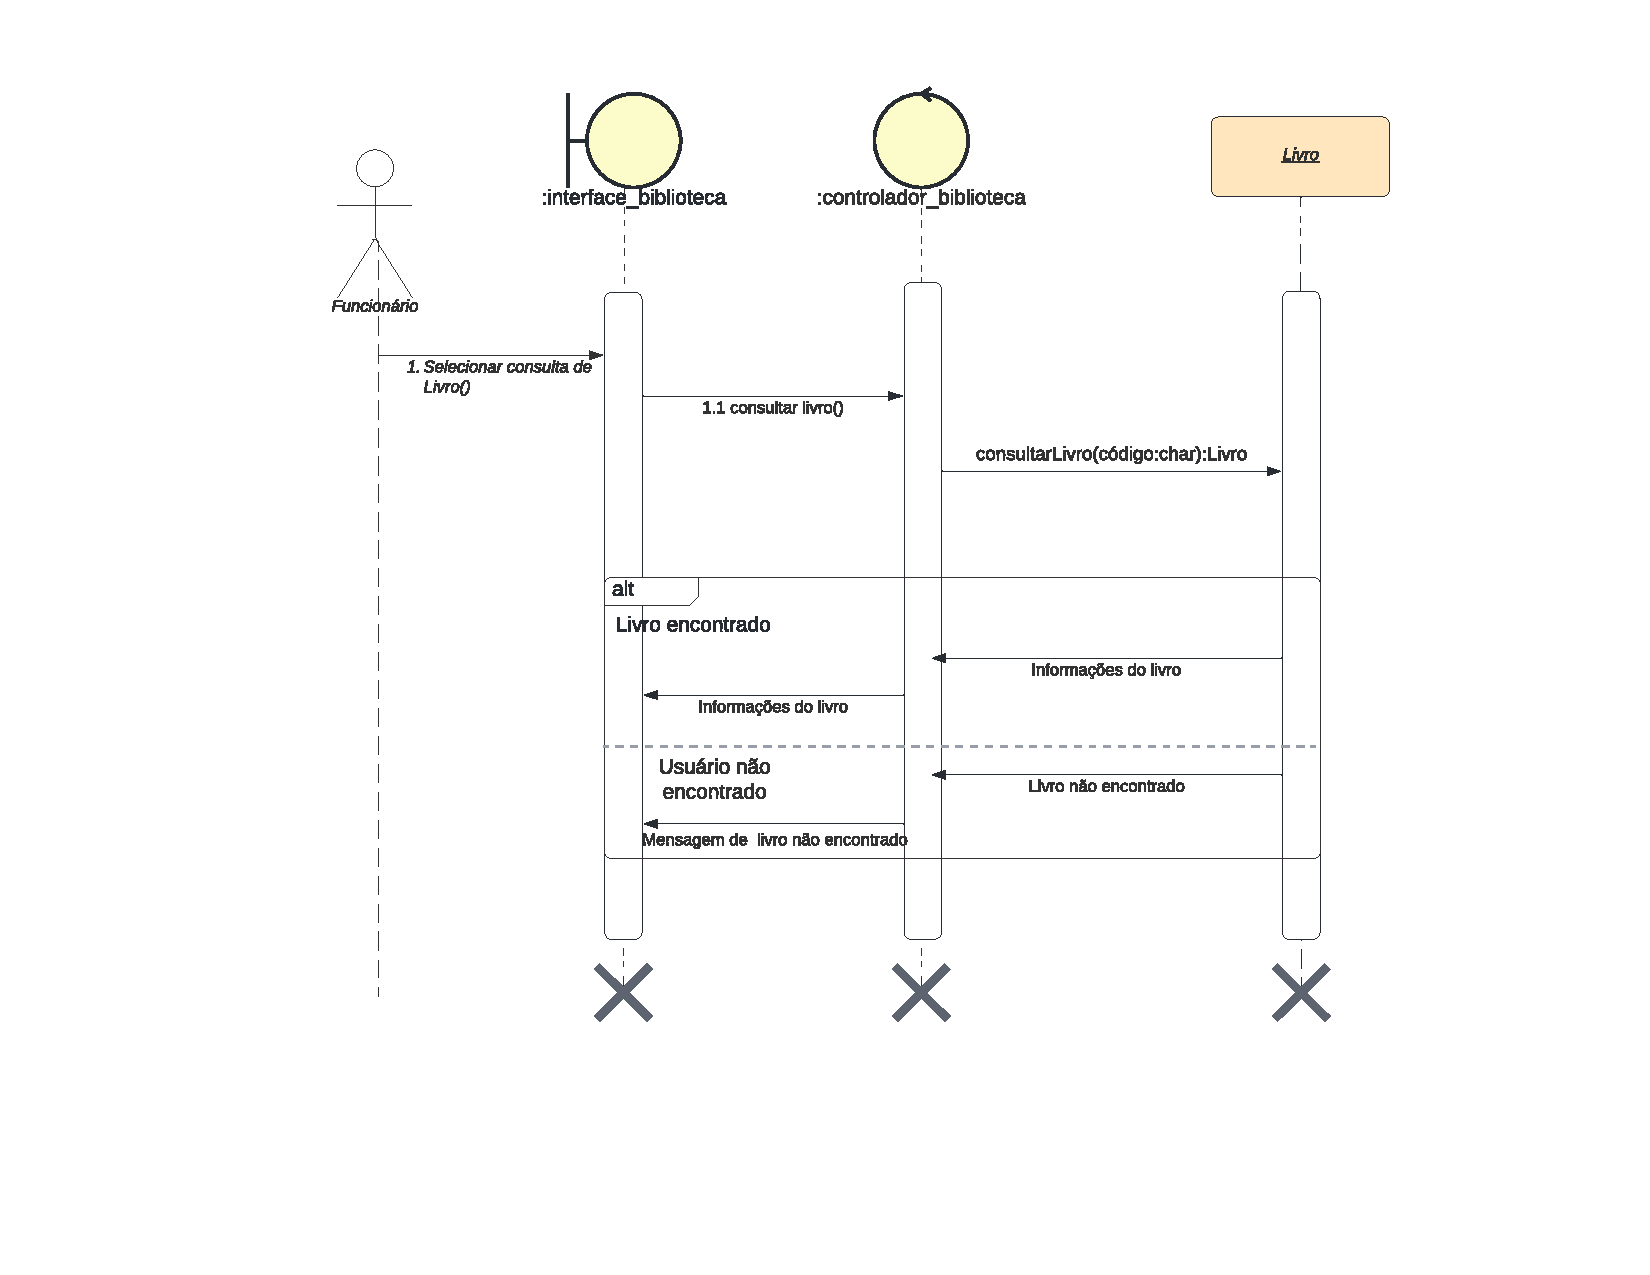
\includegraphics[width=1.0\linewidth]{Imagens/ConsultarLivro-sequência.pdf}
\end{figure}

\newpage

\subsection{Exclusão}

\begin{figure}[h]
    \centering
    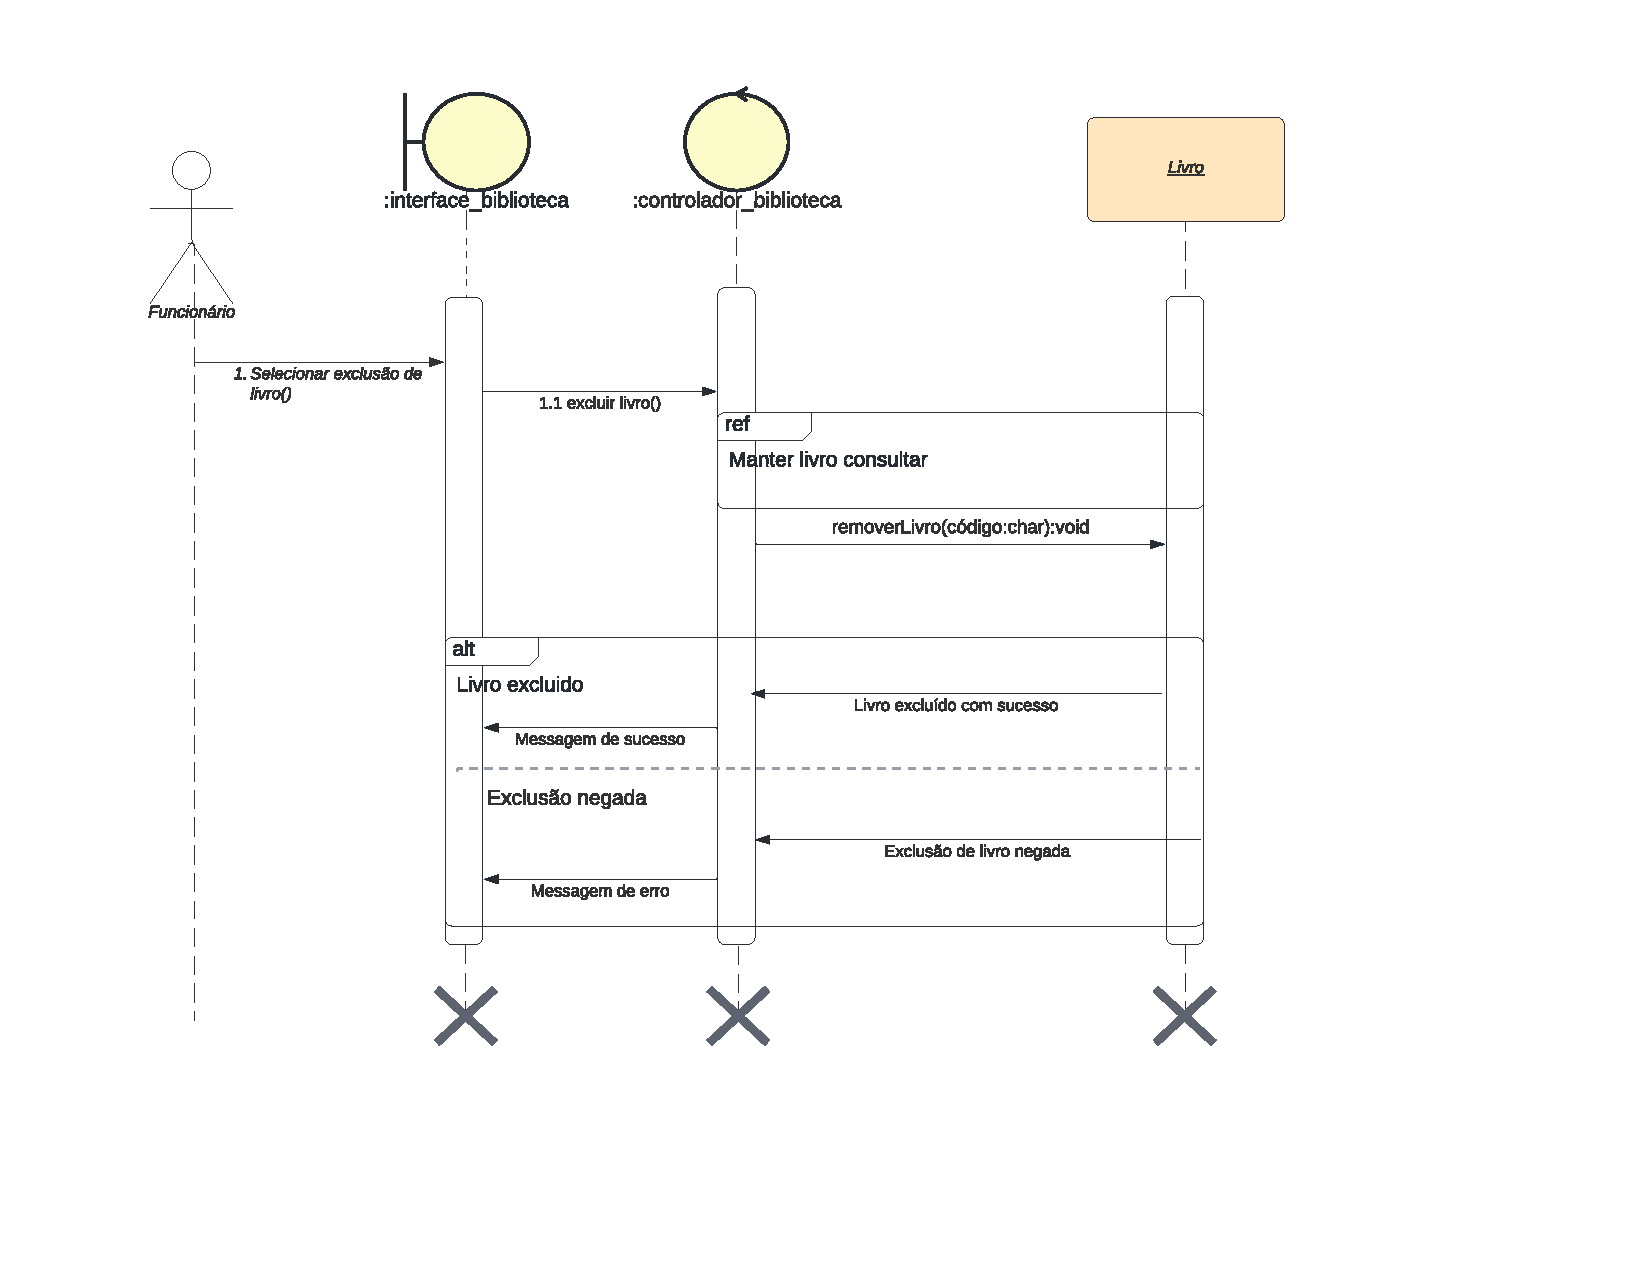
\includegraphics[width=1.0\linewidth]{Imagens/ExcluirLivro-sequência.pdf}
\end{figure}

\newpage

\subsection{Alteração}

\begin{figure}[h]
    \centering
    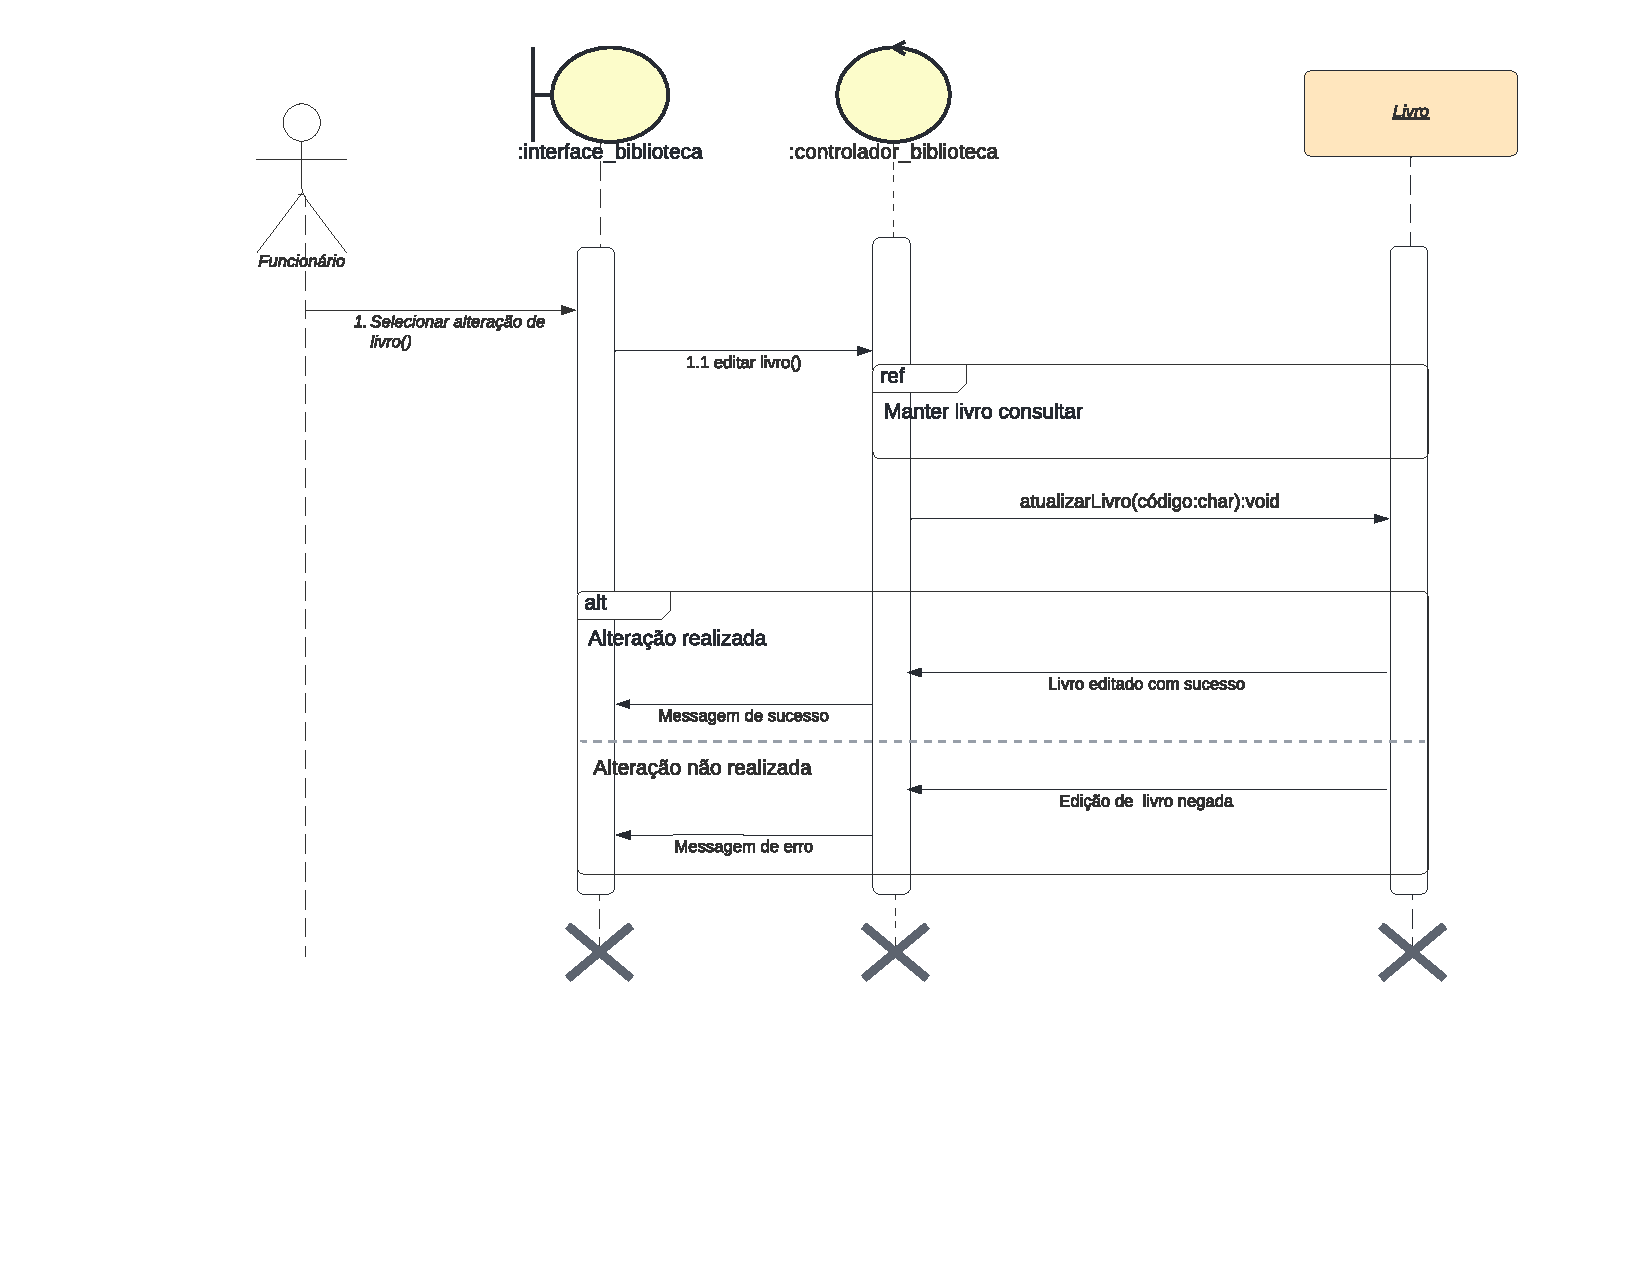
\includegraphics[width=1.0\linewidth]{Imagens/AlterarLivro-sequência.pdf}
\end{figure}

\newpage

%%%%%%%%%%%%%%%%%%%%%%%%%%%%%%%%%%%%%%%%%%%%%%%%%%%%%%%%%%%%%%%%%%%%%%%%%%%%%%%%%%%%%%%%%%%%%%%%%%%%%

\section{Manter Funcionário} 

\subsection{Cadastro}

\begin{figure}[h]
    \centering
    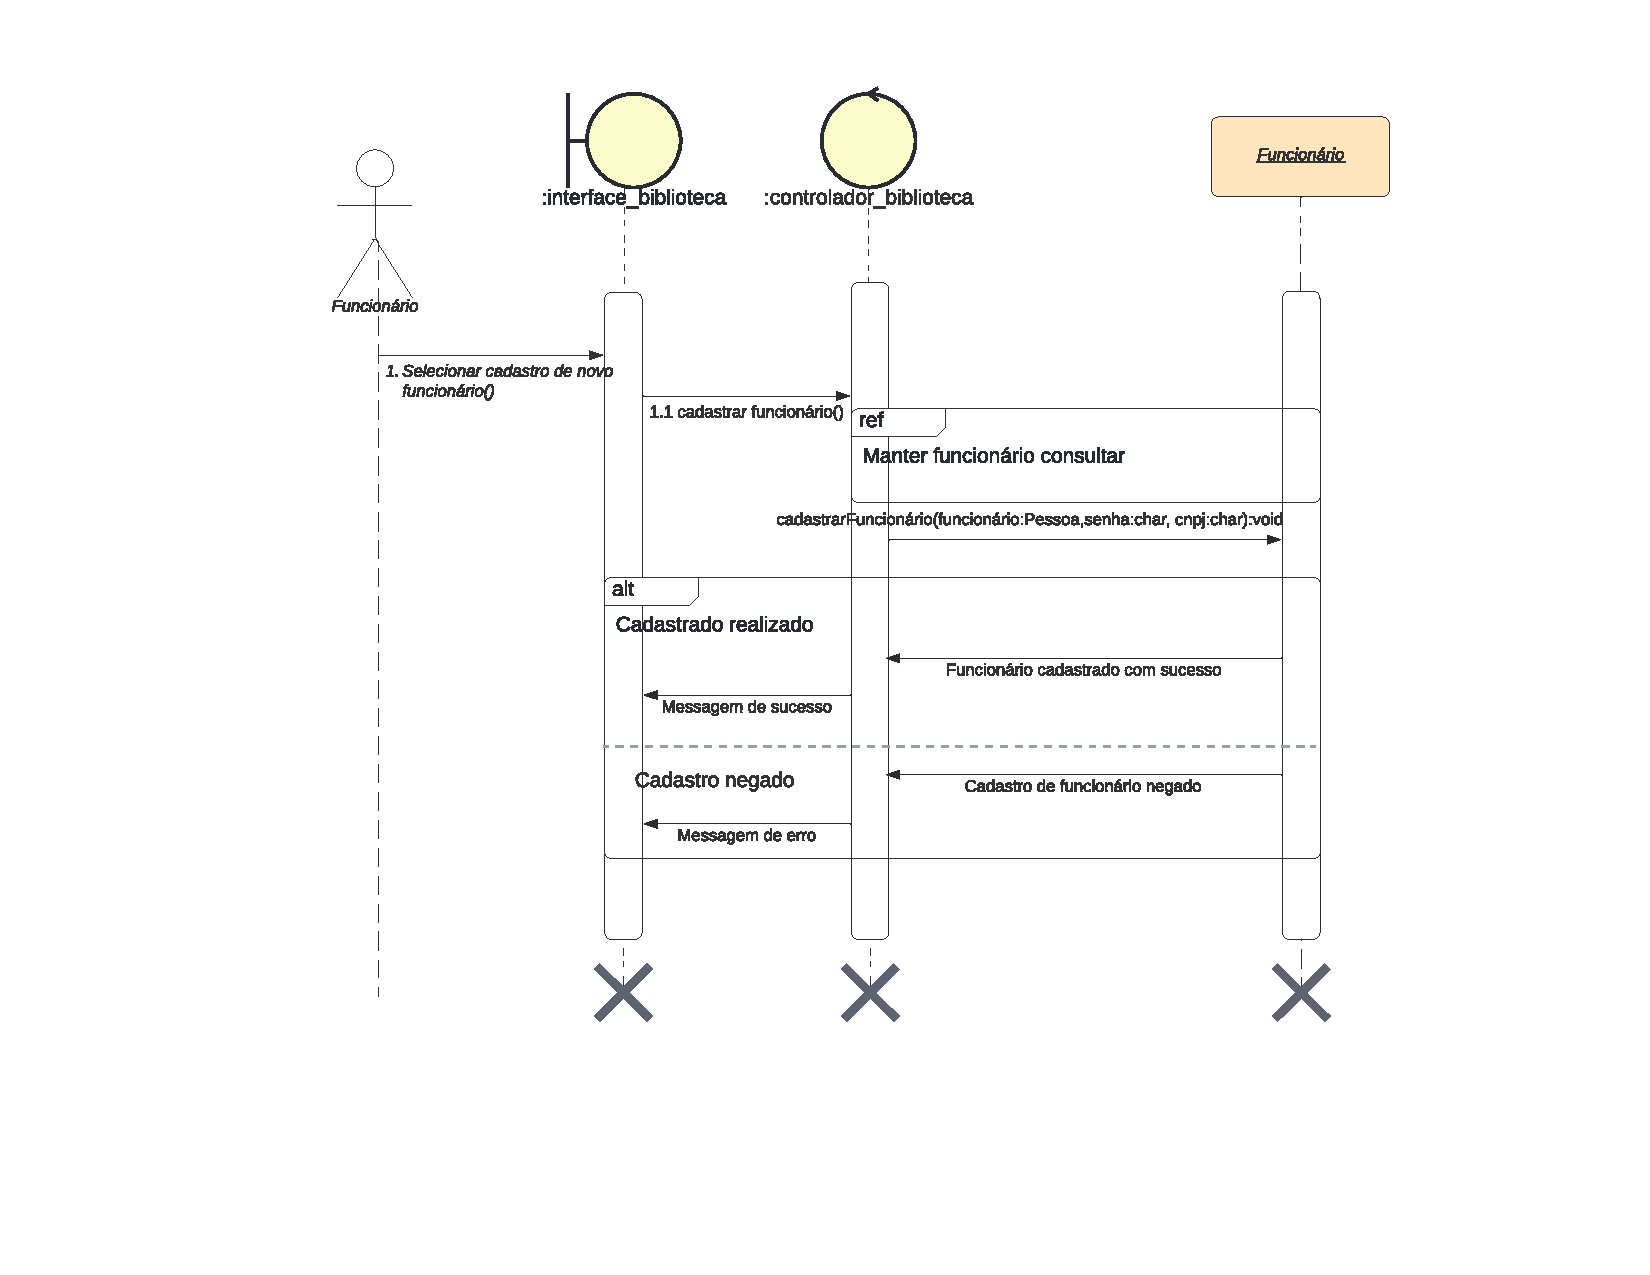
\includegraphics[width=1.0\linewidth]{Imagens/CadastrarFuncionário-sequência.pdf}
\end{figure}

\newpage

\subsection{Consulta}

\begin{figure}[h]
    \centering
    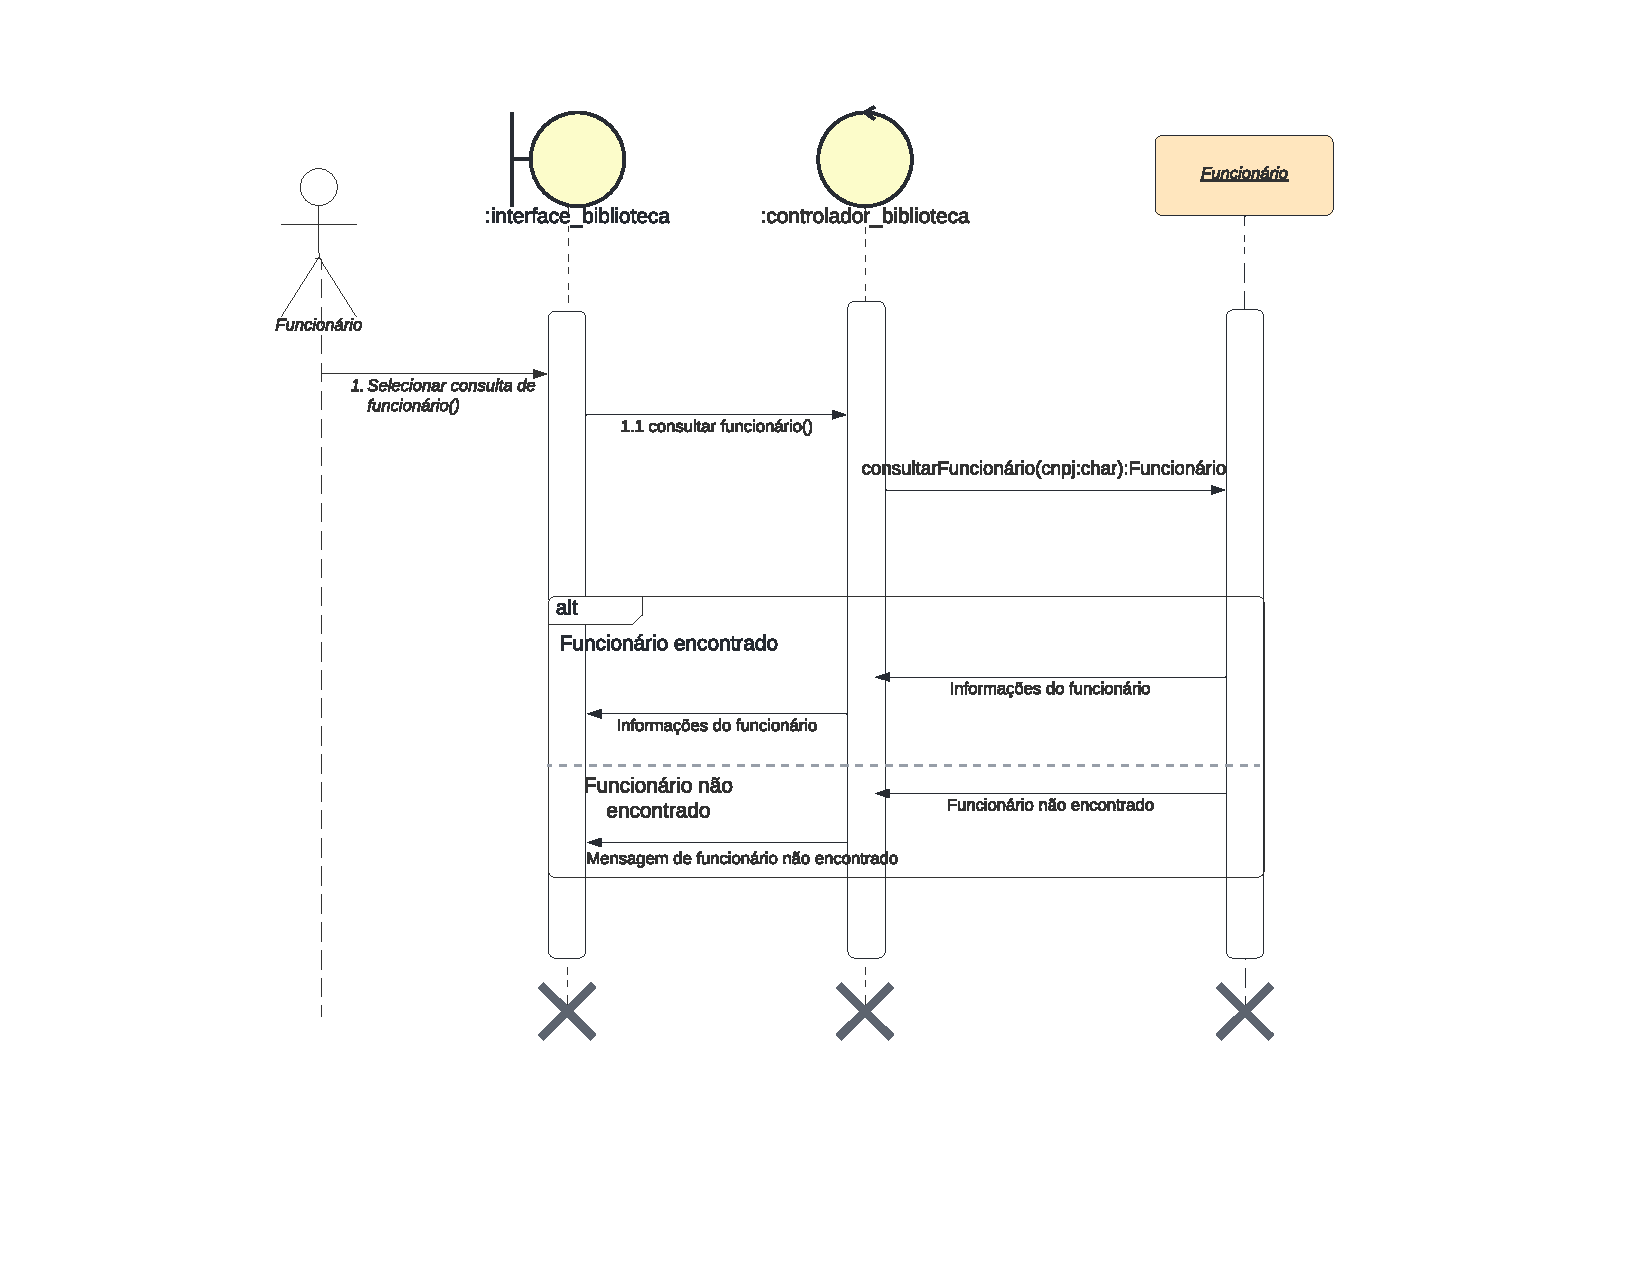
\includegraphics[width=1.0\linewidth]{Imagens/ConsultarFuncionário-sequência.pdf}
\end{figure}

\newpage

\subsection{Exclusão}

\begin{figure}[h]
    \centering
    \includegraphics[width=1.0\linewidth]{Imagens/RemoverFuncionário-sequencia.pdf}
\end{figure}

\newpage

\subsection{Alteração}

\begin{figure}[h]
    \centering
    \includegraphics[width=1.0\linewidth]{Imagens/AlterarFuncionario-sequência.pdf}
\end{figure}

		
	% Consideracoes finais
%	% Considerações finais
\chapter{Considerações finais}

As considerações finais formam a parte final (fechamento) do texto, sendo dito de forma resumida (1) o que foi desenvolvido no presente trabalho e quais os resultados do mesmo, (2) o que se pôde concluir após o desenvolvimento bem como as principais contribuições do trabalho, e (3) perspectivas para o desenvolvimento de trabalhos futuros, como listado nos exemplos de seção abaixo. O texto referente às considerações finais do autor deve salientar a extensão e os resultados da contribuição do trabalho e os argumentos utilizados estar baseados em dados comprovados e fundamentados nos resultados e na discussão do texto, contendo deduções lógicas correspondentes aos objetivos do trabalho, propostos inicialmente.


\section{Principais contribuições}

Texto.


\section{Limitações}

Texto.


\section{Trabalhos futuros}

Texto.
	
	% Bibliografia (arquivo Capitulos/Referencias.bib)
%	\bibliography{Capitulos/Referencias}
%	\bibliographystyle{abnt-alf}
	
	% Apêndice A (arquivo Includes/ApendiceA)
%	% Apêndice
\apendice
\chapter{Primeiro apêndice}

Os apêndices são textos ou documentos elaborados pelo autor, a fim de complementar sua argumentação, sem prejuízo da unidade nuclear do trabalho.
	
	% Anexo A (arquivo Includes/AnexoA)
%	% Anexo
\anexo
\chapter{Primeiro anexo}

Os anexos são textos ou documentos não elaborado pelo autor, que servem de fundamentação, comprovação e ilustração.
	
	% Página em branco
	\newpage

\end{document}